%%%%%%%%%%%%%%%%%%%%%%%%%%%%%%%%%%%%%%%%%%%%%%%%%%%%%%%%%%%%%%%%%%%%%%%%%%%%%%%
%%%%%%%%%%%%%%%%%%%%%%%%%%%%%%%%%%%%%%%%%%%%%%%%%%%%%%%%%%%%%%%%%%%%%%%%%%%%%%%
% CONTRIBUTION TO THE MESONH BOOK1:
% "A microphysical scheme for the atmospheric ice"
% Author : Jean-Pierre Pinty
% Original : 4 november, 1998
% Update   : 24 november, 1998
% March 2008, J.-P. Pinty, extension to hail
% March 2008, J.-P. Chaboureau, ice-to-snow autoconv. & editorial corrections
% May 2008, C.Lac, cloud sedimentation
%%%%%%%%%%%%%%%%%%%%%%%%%%%%%%%%%%%%%%%%%%%%%%%%%%%%%%%%%%%%%%%%%%%%%%%%%%%%%%%
%%%\documentstyle[11pt,psfig]{book}
%\documentstyle[11pt,epsf]{book}
%\setlength{\textwidth}{17.0cm}
%\setlength{\textheight}{23.0cm}
%\oddsidemargin=+1.6cm
%\evensidemargin=+0.6cm
%\voffset=-3.8cm
%\hoffset=-1.5cm
%
%\makeindex
%
%\begin{document}
%%%%%%%%%% Definition of new commands for LATEX :
%
%\def \decrefname {\par\noindent\hangindent=1truecm \hangafter=1}
%\def \decrefrule {\par\noindent{\vskip4pt\hrule width1truecm \vskip-4pt}
%                 \hangindent=1truecm \hangafter=1}
%                 \def \decfigname {\hsize= 10 cm \vglue 14 cm
%                 \par\noindent\hangindent= 1truecm \hangafter=-1}
%%
%\newcommand{\be}{\begin{equation}}
%\newcommand{\ee}{\end{equation}}
%
% >>> Mise en tete de document
% definition of a new command for the fraction :
%\newcommand{\dfrac}[2]{\frac{\displaystyle#1}{\displaystyle#2}}
%
%  definition of  new commands for the indexes :
%\newcommand{\rind}[1]{\index{#1,module MODD CST}}
%\newcommand{\see}[2]{{\it see\/}#1}
%%
%% definition of a new environment mpa and a new command \nr for the footnote that must appear for the
%%  variables in namelist EXSEG which are not read.
%% This command is not at present used.
%\renewcommand{\thefootnote}{\fnsymbol{footnote}}
%\renewcommand{\thempfootnote}{\fnsymbol{mpfootnote}}
%\renewcommand{\thefootnote}{\alph{footnote}}
%%
%%
%\baselineskip=16pt
%\parindent=25pt
%\setcounter{totalnumber}{6}
%%
%%\marginpar{\begin{flushright} Version du \date .\end{flushright}}
%%
%% Num\'erotation des pages et \'equations de type
%% <chapitre>-<num\'ero page ou \'equ.>
%%
%\setcounter{page}{1}
%\renewcommand{\theequation}{\thechapter-\arabic{equation}}
%\renewcommand{\thepage}{\thechapter-\arabic{page}}
%%
% Revision du 17/11/97
%
\chapter{Microphysical Scheme for Atmospheric Ice}\label{ICE}
\minitoc
%
\section{Introduction}
%
\subsection{Purpose of the parameterization}
%

The importance of ice microphysics to radiation transfer, energy budget and
precipitation formation in convective storms has been widely stressed until
recently (Chen and Cotton 1988; Mc Cumber et al. 1991;  Chin 1994; Caniaux
et al. 1995; Krueger et al. 1995; Yang and Houze 1995). There are several
features that differ between the liquid and the ice phase in clouds. First, the
reversible transformation between the liquid and the ice is accompagnied by a
significant latent heat release ($\sim 10\%$ of the latent heat of
condensation/evaporation), which can contribute to a further growth of convective
clouds aloft or cooling beneath by precipitating particles falling in an
unsaturated environment. Second, the terminal fall speed of the solid
hydrometeors is significantly reduced compared to that of the liquid drops of
the same weight. A direct consequence of these different aerodynamical
properties, is that a larger time scale for the life cycle of partially
glaciated convective clouds can be expected due to a larger residence time
of the solid hydrometeores and a modified spatial redistribution of
precipitations as well. Finally due to their different habit,
the light scattering properties of the ice crystals are different from those of
the cloud droplets of equivalent size and thus must be specifically accounted
for in a cloud radiative transfer scheme when the ice phase is present.

%
\subsection{Representation of the ice categories}
%

The most striking feature of the ice phase in clouds is the extreme diversity
and complexity of the crystal habits (see Pruppacher and Klett 1978) which
lead to some uncertainity in their morphological and aerodynamical properties.
This is why a great amount of curve fitting relationships have been proposed
in the past to relate a characteristic dimension of an ice crystal to its
volume, mass and terminal fall speed. So in order to elucidate the impact of
the ice phase in a mesoscale model such as {\bf Meso-NH}, many practical
arguments are in favor of unavoidable but necessary assumptions in the bulk
representation of some selected ice categories.

Actual ice parameterizations retain 2 (Rutledge and Hobbs 1983; Cotton et al.
1982\footnotemark
\footnotetext{This reference is purely historical as the CSU-RAMS ice
microphysical scheme has been greatly improved by Cotton et al. (1986)}
), 3 (Lin et al. 1983; Rutledge and Hobbs 1984; Ziegler 1985) or 4
(Ferrier 1994) and even 5 (Walko et al. 1995) ice categories. In a recent
evaluation of the impact of the number of ice categories, Mc~Cumber et al.
(1991) concluded that at least 3 different ice types are necessary to cover most
of their precipitating case study but they
draw attention on the fact that application and tuning of the scheme might be
case specific. The common agreement about an ice phase microphysical scheme is
that it must include the pristine or primary ice phase issuing from
heterogeneous nucleation processes, the aggregates or snowflakes type
corresponding to lightly rimed large ice crystals or dry assemblages
and a third category of more or less heavily rimed crystals which are
graupels, frozen drops or hail, depending of considerations on the density of
the particles. A matter of discussion can be found regarding the last category
of ice particles as a physical discrimination exists in the growth mode of
low density ($\sim 0.4$) rimed particles (assumed to be dry for the graupels)
from that of the high density ($\sim 0.9$) hailstones which grow in the wet
mode. In the definition of the present scheme, the user can handle either 3 categories of ice for simplification or 4 categories that distinguish hail from graupel.

Another point of concern is related to the supplementary prognostic equations
for the number concentration of ice crystal in each category. For instance
Cotton et al. (1986) and others use a specific equation to predict the primary
ice number concentration which is motivated by the representation of both the
heterogeneous ice-nucleation processes (see for instance, the revised version of
Meyers et al. (1992)) and the secondary production of ice crystals known as the
Hallett-Mossop (HM) or rime-splitering mechanism (Hallett annd Mossop 1974).
Furthermore, several authors (Ziegler 1985; Murakami 1990; Ferrier 1994;
Meyeers et al. 1996) have included a number concentration equation
for their precipitating ice particles in their scheme which is in contrast with
other simplified approaches where the intercept parameter of the crystal
distribution or the total number concentration is given. In the present scheme,
a somewhat different solution have been adopted. For this first version of the
scheme, neither the HM process nor the immersion freezing of cloud droplets
will be
considered at once thus giving the opportunity to simply diagnose\footnotemark
%
\footnotetext{Although there is no serious physical difficulty to consider a
prognostic equation for the primary ice total number concentration, we shall
consider this improvement in a future version of the code with a high priority.}
%
the primary ice total number in the manner described in Ferrier (1994)\footnotemark
\footnotetext{see his equation 4.33, which condenses the results of Meyers et
al. (1992)}. Secondly, rather than working with more or less
fixed number concentrations of precipitating ice or developping prognostic
equations where the shaping of the spectra by self-aggregation/break-up
processes is difficult to control, we followed Caniaux (1993) who after
compiling various published experimental observations, established that the
total number concentration $N$ can be simply related to the slope parameter
$\lambda$ of the ice precipitating category as\footnotemark
\footnotetext{The intercept parameter $N_0$ of a Marshall-Palmer law is used in
the original formulation of Caniaux (1993), but we found more convenient
to generalize the relationship in (\ref{eq1}) to the total number concentration.}:
%
\be\label{eq1}
N= C \lambda^x.
\ee
%
\noindent Taking $x=0$ means that the total number concentration is held fixed
while for $x=-1$, it is the intercept parameter ($N_0 \equiv C$) of a
Marshall-Palmer distribution law ($n(D)=N_0\,e^{-\lambda D}$) which is assumed
to be a constant. In fact, as we want to grossly reproduce the broadening of
the spectra (a decrease of $\lambda$) by the self-aggregation processes (a
reduction of $N$), it is imperative to have $x>0$.

In (\ref{eq1}), both $C$ and $x$ depend on the ice category
and must be specified from physical arguments. However, experimental evidence
and a sensitivity study leads Caniaux (1993) to link $C$ and $x$ by the
following relationship:
%
\be\label{eq2}
{\rm log_{10}}C = -3.55\,x+3.89,
\ee
%
\noindent thus reducing the degree of freedom for the choice of $C$ and $x$.

\medskip
\medskip
\noindent To summarize and as a first step toward a more advanced scheme, the
following strategy is adopted:
\begin{itemize}
\item the scheme contains a prognostic equation for the primary ice mixing ratio
$r_i$, the snowflakes mixing ratio $r_s$, and the rimed crystals mixing ratio
$r_g$,
\item the total number concentration of the primary ice $N_i$ is diagnosed
while the total number concentration of the snowflakes $N_s$ and of the rimed
crystals $N_g$ follow (\ref{eq1}),
\item power law relationships are used to relate the mass to the diameter\footnotemark
\footnotetext{The diameter $D$ refers to the maximum ice particle dimension.
From (\ref{eq3}), it is easy to show that $D_{sph}$, the equivalent spherical
diameter is $D_{sph}=(6/\pi\ a/\rho_{ice})^{1/3}D^{b/3}$ with $\rho_{ice}$ being
the density of the ice (taking $\rho_{ice}=\rho_w$ means that $D_{sph}$ is the
melted diameter).},
%
\be\label{eq3}
m(D) = aD^b
\ee
%
\noindent and the terminal speed velocity to the diameter
%
\be\label{eq4}
v(D) = cD^d \, (\rho_{00}/\rho_{dref})^{0.4},
\ee
%
\noindent where the last factor is the Foote and Du Toit (1969) correction of
the air density, $\rho_{00}$ being the air density at the reference pressure
level $P_{00}$.
\item each category of ice particle is assumed to be distributed according to
%
\be\label{eq5}
n(D) = N\,g(D),
\ee
%
\noindent where $g(D)$ is a normalized distribution law to be chosen in
Table \ref{table1}.

\begin{table}
\caption{Analytical formulation of various normalized distribution laws
(from Tripoli and al. 1988).}
\begin{center}\label{table1}
  \begin{tabular}{|l|l|}
\hline
Name of the distribution law & Mathematical expression  \\
\hline \hline
generalized Gamma & $g(D)=\frac{\displaystyle{\alpha}}{\displaystyle{\Gamma(\nu)}}
\lambda^{\alpha \nu} D ^{\alpha \nu -1} \exp\big(-(\lambda D)^{\alpha}\big)$ \\
\hline
Gamma ($\alpha=1$) & $g(D)=\frac{\displaystyle{\lambda^{\nu}}}{\displaystyle{\Gamma(\nu)}}
D^{\nu -1} \exp(-\lambda D)$ \\
\hline
Marshall-Palmer ($\alpha=1$ and $\nu=1$) & $g(D)=\lambda \, \exp(-\lambda D)$ \\
\hline
Weibull ($\nu=1$) & $g(D)=\alpha \lambda^{\alpha} D ^{\alpha -1}
\exp\big(-(\lambda D)^{\alpha}\big)$ \\
\hline
Rayleigh ($\alpha=2$ and $\nu=3/2$) & $g(D)=\frac{\displaystyle{\lambda^{3}}}
{\displaystyle{\sqrt{\pi}}} D^{2} \exp\big(-(\lambda D)^{2}\big)$ \\
\hline
Lognormal & $g(D)=\frac{\displaystyle{1}}{\displaystyle{\sqrt{2 \pi} \sigma D}}
\exp\big[-\big(\frac{\displaystyle{\log(\lambda D)}}{\displaystyle{\sqrt{2} \sigma }}
\big)^{2}\big]$ \\
\hline
  \end{tabular}
\end{center}
\end{table}

It can be noticed that according
to Tripoli and al. (1988), the use of the generalized Gamma law allows the
maximal flexibility without requiring much computation effort as for instance,
$M(p)$, the $p^{th}$ moment of the law is simply expressed as:
%
\be\label{eq6}
M(p)=\int^{\infty}_{0} \, D^{p} g(D) \, dD=\frac{\displaystyle{G(p)}}{\displaystyle{\lambda^{p}}},
\ee
%
\noindent where
%
\be\label{eq7}
G(p) = \frac{\displaystyle{\Gamma(\nu+p/\alpha)}}{\displaystyle{\Gamma(\nu)}},
\ee
%
\noindent for a generalized Gamma law or
%
\be\label{eq8}
G(p) = \exp\big(\frac{\displaystyle{p^2 \sigma^2}}{\displaystyle{2}}\big),
\ee
%
\noindent in case of lognormal distribution.
\item the ice content, $\rho r$, of any specy $i$, $s$ or $g$ is defined by:

%
\be\label{eq9}
\rho r=\int^{\infty}_{0} \, m(D) n(D) \, dD=a N M(b),
\ee
%

\noindent where (\ref{eq3}), (\ref{eq5}), and (\ref{eq6}) have been used. The
slope parameter $\lambda$ is then easily computed by inserting (\ref{eq1}) and
(\ref{eq6}) into (\ref{eq9}) to give:

%
\be\label{eq10}
\lambda = \Big(\frac{\displaystyle{\rho r}}{\displaystyle{aCG(b)}}\Big)^{\frac{\displaystyle{1}}{\displaystyle{x-b}}}.
\ee
%

Corollarily, it can be seen from the above equation that $x<b$ to ensure an
opposite sense of variation for $\rho r$ and $\lambda$ (see Fig. \ref{mixfigCaniaux})
that is the presence of large ice particles (low $\lambda$)
are associated with high mixing ratios $r$ and probably low concentration
$x>0$ as shown above.

\end{itemize}

\begin{figure}
\centerline{\includegraphics[]{\EPSDIR/Caniaux.eps}}
\caption{Modified Marshall-Palmer distribution $n(D)$ as a
function of the slope parameter $\lambda$ in log scale (from Caniaux 1993).}
\label{mixfigCaniaux}
\end{figure}

%
\subsection{General characteristics of the ice crystals}
%

Each ice category is characterized by a specific set of value for the parameters
involved in (\ref{eq1}) according to their relative size abundance and in
(\ref{eq3}; mass-diameter), (\ref{eq4}; fall speed-diameter), (\ref{DEP3};
vapor growth capacity-diameter), and (\ref{DEP4}; ventilation factor-diameter)
depending upon their habit and growth mode. Note that each ice
crystal is potentially precipitating even if the terminal fall speed of the
primary ice crystal is negligible compared to that of the aggregates and the
rimed particles. Doing so ensures the long term dissipation of unactive cirrus
clouds or thunderstorm anvils by the sublimation of crystals falling in
the subsaturated layers underneath.

Cloud ice is assumed to be distributed by a low dispersion (high $\nu$)
generalized Gamma law corresponding to an exponential distribution of the volume
of quasi-spherical crystals ($\alpha = 3$) (see, Ziegler 1985) while the
precipitating particles follow the more classical exponential (or
Marshall-Palmer) law.

\begin{table}
\caption{Set of parameters used to characterize each ice category
and the raindrops (Kessler scheme).}
\begin{center}\label{table2}
\begin{tabular}{|l|l|l|l|l|l|l|}
\hline
Parameters & $r_i$ & $r_s$ & $r_g$ && $r_r$ & $r_c$ \\
\hline \hline
$\alpha$ & 3 & 1 & 1 && 1 & 3 on sea; 1 on land \\
$\nu$    & 3 & 1 & 1 && 1 & 1 on sea; 3 on land \\
\hline
$a$ & 0.82 & 0.02 & 19.6 && 524 & 524 \\
$b$ & 2.5  & 1.9  & 2.8 && 3 & 3  \\
\hline
$c$ & 800  & 5.1  & 124 && 842 & 3.2 10$^7$ \\
$d$ & 1.00 & 0.27 & 0.66 && 0.8 & 2 \\
\hline
$C$ & & 5 & 5 10$^5$ && 8 10$^6$ & \\
$x$ & & 1 &    -0.5   &&   -1  &  \\
\hline
$\overline{f}_0$ & 1.00 & 0.86 & 0.86 && 1.00 & \\
$\overline{f}_1$ &      & 0.28 & 0.28 && 0.26 & \\
$\overline{f}_2$ & 0.14 &      &      &&      & \\
\hline
${\cal C}_{1}$ & $1/\pi$ & 1/$\pi$ & 0.5 && 0.5 & \\
\hline
\end{tabular}
\end{center}
\end{table}

In Table \ref{table2}, the parameters of the $r_s$ class describe the behavior of
unrimed radiating assemblages of plates, side planes, bullets and columns or
that of densely rimed radiating assemblages of dendrites. The parameters chosen
for the $r_g$ class correspond to those of lump graupels\footnotemark
\footnotetext{For hailstones, $a=470$ and $b=3$ corresponding to spherical
particles of density $\rho_{ice}=900$ kg/m$^3$ together with $c=207$ and
$d=0.64$ (B\"ohm 1989) and $C \sim 5\ 10^{-4}$ with $x \sim 2$ are recommended
values from the analysis made by Cheng and English (1983).}. All the values of the
$a$, $b$, $c$ and $d$ parameters are taken from Locatelli and Hobbs (1974) for
the icy hydrometeors and from Starr and Cox (1985) and Heymsfield (1972) for the
primary crystals (hexagonal plates)\footnotemark
%
\footnotetext{Starr and Cox (1985) provided several sets for $a$, $b$, $c$ and
$d$ suitable for different crystal habits in cirrus clouds. They are recalled
in the table below for completness.

\begin{center}
\begin{tabular}{|l|l|l|l|}
\hline
Crystal habit & Columns & Bullet rosettes & Plates \\
\hline \hline
$a$ & $2.14\ 10^{-3}$ & 44  & 0.82 \\
$b$ & 1.7             & 3.0 & 2.5  \\
\hline
$c$ & $2.1\ 10^5$ & $4.3\ 10^5$  & $8.0\ 10^2$ \\
$d$ & 1.585       & 1.663        & 1.000       \\
\hline
\end{tabular}
\\
\end{center}

Note that the fall speed parameters are valid for the crystal size range of
0-200 $\mu$m and that $c$ contains the air density correction ($\rho=0.58$
kg/m$^3$ assumed at 40 kPa). The bullet rosettes with a quasi spherical
shape ($b=3$) impose to take ${\cal C}_{{1}_i}$ closer to 0.5 in such a case.}.
%
The ventilation coefficients ($\overline{f}_{0,1,2}$), based on Hall and
Pruppacher (1977), are valid for spheres and for oblate spheroids as well. The
$C-x$ values have been selected after the work of Passarelli (1978) and
Mitchell (1988)\footnotemark
%
\footnotetext{Values for $x$ close to 2 have been retrieved by recent radar and
aircraft data analysis (see, Thomason et al. 1995 in $27^{\rm th}$ {\it Conf.
on Radar Met.} but for spectrum tails due to large particles). However taking
$x$ too much close to 2 leads to some inconsistancies in computing $\lambda$
from (\ref{eq10})}
%
on the snowflake distribution theory and of Houze et al. (1979), but with a
large uncertainty on the fact that the measured crystals could be graupels. It
is important to stress that $x=1$ is an acceptable value for snow because these
particles are bidimensional particles ($b=1.9$) with a variable density.


%
\subsection{Nomenclature}
%

The different rates at which microphysical processes involving one ice specy
at least, have a symbolic name which is built according to the following rules:
\begin{itemize}
\item a first letter ($R$ or $C$) to mean that the rate is relevant for a
mixing $R$atio or for a $C$oncentration,
\item a second letter ($V$, $C$, $I$, $R$, $S$ or $G$) to identify the $S$ink
specy,
\item a group of three letters to shorten the name of the $MIC$rophysical process,
\item an optional letter to recall the name of the "$R$eactant" specy in case of
three-component process,
\item a last letter ($I$, $R$, $S$ or $G$) to identify the $S$ource specy.
\end{itemize}


%
\subsection{Outlines of the microphysical scheme for mixed phase clouds}
%

%
\subsubsection{Warm processes}
%
%\vskip 1cm
\begin{table}[!ht]
\caption{List of the warm microphysical processes (not involving ice particles).}
\begin{center}\label{table5}
\begin{tabular}{|c|c|c|c|c|c|c|}
\hline
Symbol & Mechanism & Sink & Source & Process \\
\hline \hline
 & & & & \\
$RVCNDC$ & $r_v\ \Longrightarrow \ r_c$ & $r_v$ & $r_c$ & condensation on cloud droplets \\
 & & & & \\
$RCAUTR$ & $r_c+r_c\ \Longrightarrow \ r_r$ & $r_c$ & $r_r$ & autoconversion of cloud droplets \\
 & & & & \\
$RCACCR$ & $r_c+r_r\ \Longrightarrow \ r_r$ & $r_c$ & $r_r$ & accretion of cloud droplets by raindrops \\
 & & & & \\
$RREVAV$ & $r_r\ \Longrightarrow \ r_v$ & $r_r$ & $r_v$ & evaporation(condensation) \\
 & & & & \\
\hline
\end{tabular}
\end{center}
\end{table}

Cloud droplets nucleate and grow by condensation of water vapor or are forced to
evaporate instantaneously according to the supply of water vapor by transport.
Then autoconversion and accretion processes take place to form and accelerate
the growth of the precipitable raindrops which evaporate when falling below the
cloud base.

%
\newpage
\subsubsection{Cold processes}
%
%\vskip 1cm

%
\begin{table}[!ht]
\caption{List of the cold microphysical processes (involving ice particles).}
\label{table4}
\begin{center}
\begin{tabular}{|c|c|c|c|c|c|c|}
\hline
Symbol & Mechanism & Sink & Source & Process \\
\hline \hline
% & & & & \\
$RVHENI$ & $r_v\ \Longrightarrow \ r_i$ & $r_v$ & $r_i$ & heterogeneous nucleation\\
 & & & & \\
$RCHONI$ & $r_c\ \Longrightarrow \ r_i$ & $r_c$ & $r_i$ & homogeneous nucleation\\
$RRHONG$ & $r_r\ \Longrightarrow \ r_g$ & $r_r$ & $r_g$ & homogeneous nucleation\\
 & & & & \\
$RCBERI$ & $r_c\ \Longrightarrow \ r_i$ & $r_c$ & $r_i$ & Bergeron-Findeisen effect \\
 & & & & \\
$RVDEPI$ & $r_v+r_i\ \Longrightarrow \ r_i$ & $r_v$ & $r_i$ & deposition(sublimation) \\
$RVDEPS$ & $r_v+r_s\ \Longrightarrow \ r_s$ & $r_v$ & $r_s$ & deposition(sublimation) \\
$RVDEPG$ & $r_v+r_g\ \Longrightarrow \ r_g$ & $r_v$ & $r_g$ & deposition(sublimation) \\
 & & & & \\
$RIAUTS$ & $r_i+r_i\ \Longrightarrow \ r_s$ & $r_i$ & $r_s$ & autoconversion of pristine ice \\
 & & & & \\
$RIAGGS$ & $r_i+r_s\ \Longrightarrow \ r_s$ & $r_i$ & $r_s$ & aggregation of pristine ice \\
 & & & & \\
$RRCFRIG$ & $r_i+r_r\ \Longrightarrow \ r_g$ & $r_r$ & $r_g$ & raindrops contact freezing \\
$RICFRRG$ & $r_i+r_r\ \Longrightarrow \ r_g$ & $r_i$ & $r_g$ & raindrops contact freezing \\
 & & & & \\
$RCRIMSS$ & $r_c+r_s\ \Longrightarrow \ r_s$ & $r_c$ & $r_s$ & light riming of aggregates \\
$RCRIMSG$ & $r_c+r_s\ \Longrightarrow \ r_g$ & $r_c$ & $r_g$ & heavy riming of aggregates \\
$RSRIMCG$ & $r_c+r_s\ \Longrightarrow \ r_g$ & $r_s$ & $r_g$ & heavy riming of aggregates \\
 & & & & \\
$RRACCSS$ & $r_r+r_s\ \Longrightarrow \ r_s$ & $r_r$ & $r_s$ & accretion of rain and aggregates \\
$RRACCSG$ & $r_r+r_s\ \Longrightarrow \ r_g$ & $r_r$ & $r_g$ & accretion of rain and aggregates \\
$RSACCRG$ & $r_r+r_s\ \Longrightarrow \ r_g$ & $r_s$ & $r_g$ & accretion of rain and aggregates \\
 & & & & \\
$RCDRYG$ & $r_c+r_g\ \Longrightarrow \ r_g$ & $r_c$ & $r_g$ & dry growth of the graupels \\
$RIDRYG$ & $r_i+r_g\ \Longrightarrow \ r_g$ & $r_i$ & $r_g$ & dry growth of the graupels \\
$RRDRYG$ & $r_r+r_g\ \Longrightarrow \ r_g$ & $r_r$ & $r_g$ & dry growth of the graupels \\
$RSDRYG$ & $r_s+r_g\ \Longrightarrow \ r_g$ & $r_s$ & $r_g$ & dry growth of the graupels \\
 & & & & \\
$RCWETG$ & $r_c+(r_g)\ \Longrightarrow \ r_r$ & $r_c$ & $r_r$ \& $r_g$ & partial freezing \& water shedding \\
$RRWETG$ & $r_r+(r_g)\ \Longrightarrow \ r_g$ & $r_r$ & $r_g$ & partial freezing
\& water shedding \\
$RIWETG$ & $r_i+r_g\ \Longrightarrow \ r_g$ & $r_i$ & $r_g$ & wet growth of the graupels \\
$RSWETG$ & $r_s+r_g\ \Longrightarrow \ r_g$ & $r_s$ & $r_g$ & wet growth of the graupels \\
 & & & & \\
$RIMLTC$ & $r_i\ \Longrightarrow \ r_c$ & $r_i$ & $r_c$ & melting \\
$RGMLTR$ & $r_g\ \Longrightarrow \ r_r$ & $r_g$ & $r_r$ & melting \\
$RSCVMG$ & $r_s\ \Longrightarrow \ r_g$ & $r_s$ & $r_g$ & conversion melting \\
% & & & & \\
\hline
\end{tabular}
\end{center}
\end{table}

Small ice crystals are initiated by two heterogeneous nucleation processes:
\begin{itemize}
\item deposition: formation of ice embryos in a supersaturated environment over
ice,
\item contact: freezing of supercooled droplet subsequent to the attraction of
aerosol particles by Brownian motion or by phoretic diffusion (a function of
temperature).
\end{itemize}

Also, when the temperature drops below $-35^\circ$C, the homogeneous nucleation or
droplet freezing takes place to deplete very rapidly the cloud droplets.

Ice crystals can grow by water vapor deposition or decay by sublimation
depending on the level of saturation of the environment with respect to ice.
Aggregates are formed by autoconversion process of pristine ice crystals while
the primary source of graupel is either raindrop contact freezing or heavy
riming of the snowflakes. When the air temperature is warmer than $T_t$, the
small primary ice crystals are immediately converted into cloud water, the
snowflakes are transfered into the graupel category at a rate proportional to
their partial melting (Walko et al. 1995) and finally the graupels melt by
shedding all the liquid water into raindrops.

The representation of ice crystal growth by collection processes (for instance
by aggregation, riming or rain contact freezing) remains the most difficult and
controversial task. As in many bulk parameterizations, the assumptions of
continuous growth and the simple geometric sweep-out concept for the collection kernel $K$ are retained.
So the mutual gravitational interaction between
species $X$ and $Y$ leads to a general definition of $K$,
%
\be\label{ACC1}
K(D_x,D_y)=\frac{\displaystyle{\pi}}{\displaystyle{4}}(D_x+D_y)^2 |v_x(D_x)-v_y(D_y)| E_{xy},
\ee
%
\noindent where $E_{xy}$ is the collection efficiency (often, a poorly known
quantity).

In the most general case, the collection process $COL$ involving $X$ and $Y$
can lead to the formation of a third specy $Z$ (simultaneous collection and
conversion processes with sometimes further external conditions on the mixing
ratios $r_x$ and $r_y$), so the mixing ratio tendency of specy $Y$ (a loss for
$Y$) due to the mass collection of $X$ is:
%
\be\label{ACC2}
RYCOLXZ= \rho^{-1} \int_{0}^{\infty} \Big\{ \int_{0}^{\infty} K(D_x,D_y)\ m_y(D_y)n_y(D_y)dD_y) \Big\} n_x(D_x)dD_x,
\ee
%
\noindent conversely the mixing ratio tendency for $X$ (a loss too but for $X$) is:
%
\be\label{ACC3}
RXCOLYZ= \rho^{-1} \int_{0}^{\infty} \Big\{ \int_{0}^{\infty} K(D_x,D_y)\ m_x(D_x)n_x(D_x)dD_x \Big\} n_y(D_y)dD_y,
\ee
%
\noindent and the  mixing ratio tendency of specy $Z$ (a gain for $Z$) is simply
$RXCOLYZ+RYCOLXZ$.
When $Z$ identifies to one of the initial specy $X$ or $Y$, i. e. a two
component process, a single mixing ratio collection rate needs to be computed as
for instance Eq. (\ref{ACC3}) if $Z \equiv Y$ or Eq. (\ref{ACC2}) if $Z \equiv X$
as for instance
%
\be\label{ACC3prime}
RYCOLX= \rho^{-1} \int_{0}^{\infty} \Big\{ \int_{0}^{\infty} K(D_x,D_y)\ m_y(D_y)n_y(D_y)dD_y) \Big\} n_x(D_x)dD_x=-RXCOLY
\ee
%
\noindent is the mixing ratio rate of change of specy $X$ due to the single
collection of specy $Y$.


More complicated and as discussed by Farley et al. (1989) and Ferrier (1994),
collection processes might be envisionned as both two and three component
processes when threshold diameters are introduced for instance to convert specy
$Y$ into specy $Z$ if and only if the diameter $D_y$ of $Y$ is larger than a
required value $D_y^{lim}$. This means than only a fraction
(generally the upper diameter one) of specy $Y$,
collecting specy $X$, will be converted into specy $Z$ and thus be removed from
the $Y$ category, while the remaining fraction of the former specy $Y$ increases
its mass as a binary collection process between $X$ and $Y$. So, the growth of
$X$ from $Y$ is now:
%
\be\label{ACC4}
RYCOLXX= \rho^{-1} \int_{0}^{\infty} \Big\{ \int_{0}^{D_y^{lim}}
K(D_x,D_y)\ m_y(D_y)n_y(D_y)dD_y) \Big\} n_x(D_x)dD_x,
\ee
%
\noindent the growth of $Z$ from both $X$ and $Y$ is:
%
\be\label{ACC5}
\begin{array}{rl}
RYCOLXZ&=RYCOLX-RYCOLXX \\
       &=\rho^{-1} \displaystyle{\int_{0}^{\infty}} \Big\{
                   \displaystyle{\int_{D_y^{lim}}^{\infty}}
K(D_x,D_y)\ m_y(D_y)n_y(D_y)dD_y) \Big\} n_x(D_x)dD_x, \\
\end{array}
\ee
%
\noindent while $RYCOLX$, the total loss of $Y$ (leading to the growth of $X$ in
Eq. (\ref{ACC4}) and to the growth of $Z$ in Eq. (\ref{ACC5})), is given by
Eq. (\ref{ACC3prime}).

Although, this approach has much more physical basis, it needs a (technically
more complicated) partial integration over the dimensional spectrum of at least
a specy to compute the mixing ratio tendencies.

In the present parameterization, any accreted material on the graupels cannot
change the type of this crystal but the concurrent dry/wet growth regimes will
compete in the manner described by Lin et al. (1983). So much of these
collection processes will be described by integrals of type (\ref{ACC3prime}).
Considering now the collection processes on aggregates, it is postulated that
beyond a critical size of the initial aggregate, the riming of cloud droplets
may modify so much the crystal characteristics that it is converted into a
graupel. Furthermore, the collection of raindrops on aggregates is also very
efficient to convert the upper part of the aggregate spectrum into graupels in
the manner suggested by Ferrier (1994). So partial integrals of the form
(\ref{ACC4}) need to be computed to represent the two latter collection processes.

%\vfill
\newpage
%
\section{Microphysical processes}
%
%
\subsection{Summary of the scheme}
%
%See Fig. \ref{mixfigdiagram}
\begin{figure}[!ht]
\centerline{\includegraphics[]{\EPSDIR/diagram.eps}}
\caption{Diagram of the microphysical processes for mixed phase cloud in the present scheme.}
\label{mixfigdiagram}
\end{figure}

%
\subsection{Warm processes}
%\subsection{Warm processes: $RCAUTR$, $RCACCR$ and $RREVAV$}
%
The parameterization of these processes is borrowed from the widespread Kessler
scheme described elsewhere, so the mathematical expression of these processes is
only recalled here for completness.

%
\be\label{WARM1}
RCAUTR=k_{cr}\ Max(0,r_c-r_c^*),
\ee
%
\noindent with $k_{cr}=10^{-3}$ s$^{-1}$ and
$q_c^*=r_c^*/\rho_{dref}=0.5\ 10^{-3}$ kg/m$^3$.

%
\be\label{WARM2}
RCACCR=\dfrac{\pi}{4} N_r r_c c_r M(d_r+2)
\Big( \frac{\displaystyle{\rho_{00}}}{\displaystyle{\rho_{dref}}} \Big)^{0.4}
\ee
%
\noindent and
%
\be\label{WARM3}
RREVAV=\dfrac{4\pi}{\rho} \dfrac{(-SS_{w})}{A_{w}(T,P)} N_r {{\cal C}_1}_r
    \big[{\overline{f}_0}_r M_r(1)+
         {\overline{f}_1}_r c^\prime_r M_r(\dfrac{d_r+3}{2})
    \big],
\ee
%
\noindent where $SS_w=r_v/r_{vs_{w}}-1$ and
$$
A_{w}(T,P)=\dfrac{L_v(T)^2}{k_a(T) R_v T^2}+\dfrac{R_v T}{D_v(T,P) e_{sw}(T)}.
$$
\noindent ${{\cal C}_1}_r$, ${{f}_0}_r$ and ${{f}_1}_r$ are taken from
Table \ref{table2} and
$c^\prime_r=Sc_{v}^{1/3}(c_r \rho/\eta)^{1/2}(\rho_{00}/\rho_{dref})^{0.2}$ with
$Sc_{v} \sim 0.635$ (see after (\ref{DEP4})). Note that according to the
nomenclature and sign convention: $RREVAV > 0$ in case of rain evaporation.

In order to reproduce the small drizzle of the fog necessary for its dissipation, the sedimentation of cloud droplets $RSEDC$ can be taken into account. The slope parameter for the cloud $\lambda_c$ used for the mass sedimentation rate is defined by :

$$
\lambda_{c} = \left\lbrack \frac{\pi}{6}\rho_{w}\frac{\Gamma (\nu_{c} + \frac{3}{\alpha_{c}})}{\Gamma (\nu_{c})}\frac{N_{c}}{\rho_{d}r_{c}} \right\rbrack ^{\frac{1}{3}}
$$

\noindent $\alpha_{c}$, $\nu_{c}$ and $N_{c}$ are defined according to the fractions of sea and land surface cover of the grid mesh, with $N_{c_{sea}}=$100~cm$^{-3}$ and $N_{c_{land}}=$300~cm$^{-3}$.
%
\subsection{Heterogeneous nucleation}
%\subsection{Heterogeneous nucleation: $RVHENI$}
%
As in Ferrier (1994) and according to Meyers et al. (1992), the number
concentration of primary ice crystals $N_{NU}$ formed by heterogeneous
nucleation is given by:

\begin{equation}\label{NU1}
  N_{NU}=\left\{ \begin{array}{ll}
                   N_{NU1}, & T-T_t \ge -5{\rm K}, \\
                   N_{NU2}, & T-T_t <   -5{\rm K}  \\
                 \end{array}
         \right.
\end{equation}
\noindent where
\begin{eqnarray}\label{NU2}
N_{NU1} &=& N_{NU1_0} \left[ (r_v-r_{vs_{i}})/(r_{vs_{w}}-r_{vs_{i}})
                     \right]^{\alpha_1} \, exp(-\beta_1(T-T_t)), \\
N_{NU2} &=& N_{NU2_0} \, exp(\alpha_2 SS_i - \beta_2),
\end{eqnarray}
\noindent where $SS_i=r_v/r_{vs_{i}}-1$ is the supersaturation ratio with
respect to ice and $r_{vs_{w}}$ is the saturated mixing ratio over supercooled
water.

Assuming that $N_i=N_{NU}$ (because the secondary ice production is not yet
considered) and for $m_{NU_0}$, the mass of a nucleated ice crystal, the mass
nucleation rate $RVHENI$ equals to:

%
\be\label{NU3}
RVHENI=(\rho \Delta t)^{-1} m_{NU_0} Max(N_{NU}-N_i^{t-\Delta t},0).
\ee
%

The typical values of the unknown parameters are given in Table \ref{table3}.

\begin{table}
\caption{Set of parameters used to parameterize the nucleation processes (from Ferrier 1994).}
\begin{center}\label{table3}
\begin{tabular}{|c|c|c|c|c|c|c|}
\hline
$N_{NU1_0}$ & $N_{NU2_0}$ & $\alpha_1$ & $\beta_1$& $\alpha_2$ & $\beta_2$ & $m_{NU_0}$  \\
\hline \hline
 & & & & & & \\
50 m$^{-3}$ & 1000 m$^{-3}$ & 4.5 & 0.6 K$^{-1}$ & 12.96 & 0.639 & $6.88\ 10^{-13}$ kg \\
 & & & & & & \\
\hline
\end{tabular}
\end{center}
\end{table}

In (\ref{NU3}), the previous ice crystal concentration $N_i^{t-\Delta t}$ is
available because the diagnostic variable $N_i=N_{NU}$ is stored after an
update by the mean of (\ref{NU1}).

%
\subsection{Homogeneous nucleation}
%\subsection{Homogeneous Nucleation: $RCHONI$ and $RRHONG$}
%
When the temperature drops below $-35^\circ$C, the spontaneous freezing of cloud
droplets in absence of ice nuclei (the homogeneous nucleation) is an active
process to convert any remaining small droplets into pristine crystals. This is
an essential process in cirriform clouds so it needs to be modeled accurately in
such cases.

The probability ${\cal P}$ of a water droplet of volume $V$ to freeze in the
interval of time $[t,\ t+\Delta t]$ is governed by the nucleation formula
%
\be\label{HOM1}
{\cal P} = 1 -\exp\Big( -\int_{t}^{t+\Delta t} J_{HOM}(T) V\ dt\Big),
\ee
%
\noindent where $V$ is the droplet volume and $J_{HOM}(T)$ the freezing rate,
tabulated by Pruppacher (1995) and reported in Table \ref{table3prime}\footnotemark
%
\footnotetext{Note that $J_{HOM}$ goes to infinity as $T-T_t<-44$ K},

%
\begin{table}
\caption{Values of $J_{HOM}(T)$ after Pruppacher (1995).}
\begin{center}\label{table3prime}
\begin{tabular}{|c|c|c|c|c|c|c|}
\hline
$T-T_t$ (K)  & -35 & -36 & -37 & -38 & -39 \\
\hline
$J_{HOM}$ (m$^{-3}$s$^{-1}$) & $2\ 10^{11}$ & $1\ 10^{13}$ & $3\ 10^{14}$ & $5\
10^{15}$ & $9\ 10^{16}$ \\
\hline
\multicolumn{6}{c}{}\\
\hline
$T-T_t$ (K)  & -40 & -41 & -42 & -43 & -44 \\
\hline
$J_{HOM}$ (m$^{-3}$s$^{-1}$) & $1\ 10^{18}$ & $2\ 10^{19}$ & $1\ 10^{21}$ & $5\ 10^{2
2}$ & $2\ 10^{23}$ \\
\hline
\end{tabular}
\end{center}
\end{table}
%
\noindent The above set of data has been approximated by a fitting curve which
is:
%
\be\label{HOM2}
J_{HOM}=\exp(\alpha_3(T-T_t)-\beta_3),
\ee
%
\noindent with $\alpha_3=-3.075$ K$^{-1}$ and $\beta_3=81.00356$.

Considering $J_{HOM}(T)$ and $V$ as constant during the timestep
$\Delta t$, (\ref{HOM1}) can be reduced to
%
\be\label{HOM3}
{\cal P} \approx J_{HOM}(T) V \Delta t.
\ee
%
Integrating (\ref{HOM3}) over the cloud droplet spectrum and differentiating
with respect to time and using (\ref{eq9}) with an appropriate form for the
cloud droplets, gives the final homogeneous nucleation rate
%
\be\label{HOM4}
RCHONI = Min \Big\{\frac{\displaystyle{r_c}}{\displaystyle{\Delta t}},
           \frac{\displaystyle{\pi}}{\displaystyle{6}}
           J_{HOM}(T) (\rho r_c)
           \frac{\displaystyle{M_c(6)}}{\displaystyle{M_c(3)}}\Big\}.
\ee
%

To compute the $M_c$ ratio in (\ref{HOM4}), it is assumed that
$\lambda_c=1.1\ 10^5$ m$^{-1}$
corresponding to a cloud droplet number concentration $N_c \sim 400\ 10^6$
m$^{-3}$ and a mixing ratio $r_c \sim 10^{-3}$ kg/kg for $\rho \sim 1$ kg/m$^3$.

Because the scheme assumes that the ice crystal concentration is determined by
the only heterogeneous nucleation parameterization, the diagnostic concentration
of these pristine crystals is not modified by the present homogenous nucleation
scheme. This is a source of error indeed because this concentration must be
accounted for in computing the very slow speed of sedimentation of cirrus clouds
in long lived simulations. The solution which has been adopted in the present
scheme employs a specific ice crystal number concentration relationship to
compute a sedimentation flux of these small crystals (see the subsection
relative to the computation of $RSEDI$).

We assume also that the raindrops cannot survive to temperature colder than
$-35^\circ$C because they are spontaneously converted to graupels by homogenous
freezing (nucleation)
%
\be\label{HOM5}
RRHONG = \frac{\displaystyle{r_r}}{\displaystyle{\Delta t}} H(T_t-35),
\ee
\noindent where $H(x)$ is the Heaviside distribution ($H(x)=0$ if $x<0$ and
$H(x)=1$ if $x \ge 0$)


%
\subsection{Deposition (sublimation) of water vapor}
%\subsection{Deposition(Sublimation) of water vapor:  $RVDEPS$ and
%$RVDEPG$}
%

The rate of mass growth or decay of a single aggregate or graupel particle by
vapor deposition or sublimation can be written as:

%
\be\label{DEP1}
\partial m/ \partial t \mid_{DEP/SUB}=4 \pi SS_i {\cal C} \overline{f} /A_{i}(T,P),
\ee
%

\noindent where $\cal C$ is the capacity of the ice crystal, $\overline{f}$ is a
ventilation factor and $A_{i}(T,P)$ is a thermodynamic function:

%
\be\label{DEP2}
A_{i}(T,P)= \frac{\displaystyle{L_s(T)^2}}{\displaystyle{k_a(T) R_v T^2}} +
        \frac{\displaystyle{R_v T}}{\displaystyle{D_v(T,P) e_{si}(T)}},
\ee
%

\noindent where $e_{si}$ is the saturation vapor pressure over ice:

\begin{equation}
e_{si}(T)= exp \big( \alpha_i - {\beta_i \over T} - \gamma_i \ln (T) \big),
\end{equation}
with
\begin{eqnarray}
&\alpha_i   &= \ln (e_{si}(T_t))+{\beta_i \over T_t} - \gamma_i \ln (T_t) \\
&\beta_i   &= {L_s(T_t) \over R_v}\gamma_i T_t \\
&\gamma_i  &= {C_i -C_{pv} \over R_v}
\end{eqnarray}

\noindent and $L_s$ is the latent heat of sublimation:
\begin{equation}
L_s(T) = L_s(T_t) + (C_{pv} - C_i)(T-T_t).
\end{equation}

\noindent The thermal conductivity of the air $k_{a}(T)$ and the diffusivity of
water vapor in the air $D_{v}(T,P)$ are given by (see Pruppacher and Klett 1978, pp. 418 and 413):

\begin{eqnarray}
D_v(T,P)&=&0.2138\ 10^{-4}(T/T_t)^{1.94}(P_{00}/P), \\
k_a(T) &=& 2.38\ 10^{-2}+0.0071\ 10^{-2}(T-T_t).
\end{eqnarray}

\noindent In (\ref{DEP1}), $\cal C$ and $\overline{f}$ have the following
expressions depending upon the crystal shape and size
%
\begin{eqnarray}\label{DEP3}
%  \cal C=\left\{ \begin{array}{ll}
%            D/\pi, & {\rm for\ disk\ like\ crystals}:\ r_i {\rm\ and\ } r_s, \\
%            D/2  , & {\rm for\ spherical\ particles}:\ r_g  \\
%                \end{array}
%         \right.
  {\cal C}= {\cal C}_{1}D
\end{eqnarray}
\begin{eqnarray}\label{DEP4}
%  \overline{f}=\left\{ \begin{array}{ll}
%            1+0.14\,X, & {\rm for\ disk\ like\ small\ crystals}:\ r_i, \\
%            0.86+0.28\,X, & {\rm for\ disk\ like\ large\ crystals}:\ r_s, \\
%            0.78+0.308\,X  , & {\rm for\ spherical\ particles:}\ r_g  \\
%                \end{array}
%         \right.
  \overline{f}=\overline{f}_{0}+\overline{f}_{1}{\chi}+\overline{f}_{2}{\chi}^2
\end{eqnarray}
%
\noindent where ${\chi}=Sc^{1/3}_{v}Re^{1/2}$ is a function of
$Sc_v=\nu(T,P)/D_{v}(T,P)$, the Schmidt number for water vapor and of
$Re=v(D)D\rho/\eta(T)$, the Reynolds number of the flow around a crystal of
size $D$. The dynamic viscosity $\eta(T)=\rho(T,P) \nu(T,P)$ of the air of
density $\rho(T,P)$ is given by (see Pruppacher and Klett 1978, p. 323):

\begin{eqnarray}
\eta(T)=1.718\ 10^{-5}+0.0049\ 10^{-5}(T-T_t).
\end{eqnarray}

\noindent In the following, $Sc_v\approx0.635$ with a very good approximation.

In \ref{DEP3}, a cylindrical shape is assumed for
the aggregates while the rimed particles are spherical (see Table \ref{table2}).
Furthermore, as the pristine ice category is assumed to contain small crystals
only, in contrast to the aggregates and rimed particles which are rather
large-size hydrometeors, the formulas of Hall and Pruppacher (1977) have been
split for a simplified application to the $D < 70 \mu$m range, relevant of the
$r_i$ specy (see below for the parameterization of the Bergeron-Findeisen
effect), and for the $D > 70 \mu$m range corresponding to the $r_s$ and
$r_g$ categories (see Table \ref{table2}).

Integration of (\ref{DEP1}) over the whole particle spectral range gives for
$X(=j)$ being $S(=s)\ $or $G(=g)$:

\be\label{DEP5}
RVDEPX=\frac{\displaystyle{4\pi}}{\displaystyle{\rho}}
    \frac{\displaystyle{SS_{i}}}{\displaystyle{A_{i}(T,P)}}
    N_j {{\cal C}_1}_j
    \big[{\overline{f}_0}_j M_j(1)+
         {\overline{f}_1}_j c^\prime_j M_j(\frac{\displaystyle{d_j+3}}{\displaystyle{2}})+
         {\overline{f}_2}_j c^{\prime 2}_j M_j(d_j+2)
    \big],
\ee

\noindent where
$c^\prime_j=Sc_{v}^{1/3}(c_j \rho/\eta)^{1/2}(\rho_{00}/\rho_{dref})^{0.2}$ and
where the moments $M_j$ of the ice category $_j$ can be expanded according to
(\ref{eq6}.)

Although the water vapor exchanges over the pristine ice crystals (and the
cloud droplets) in the present scheme are treated implicitly by an adjustment
process (see paragraph \ref{VAPADJ}), an expression equivalent to the explicit
rate $RVDEPX$ needs to be computed for the purpose of parameterizing the
Bergeron-Findeisen effect described hereafter.

%
\subsection{Bergeron-Findeisen effect}
%\subsection{Bergeron-Findeisen effect: $RCBERI$}
%
A mixed phase cloud is characterized by the simultaneous existence of cloud
droplets and small ice crystals in equilibrium with the vapor saturation level
over liquid water and ice water, respectively (Fig. \ref{mixfigBergeron}).
As the later is always lower
that the former ($e_{si}(T) < e_{sw}(T)$), there is a systematic evaporation of
the cloud droplets for deposition onto the ice crystals. This process is
independent of the droplet and crystal growth or decay due to the supply or
deficit of water vapor as for instance by vertical transport.

\begin{figure}[!ht]
\centerline{\includegraphics[]{\EPSDIR/Bergeron.eps}}
\caption{Illustration of the Bergeron-Findeisen effect and its parameterization.}
\label{mixfigBergeron}
\end{figure}

In the present scheme, it is assumed that $RCBERI$, the resulting rate of mass
transfer from the cloud droplets to the ice crystals, is determined by the rate
of water vapor deposition onto the pristine ice crystals. This rate is assumed
to be equal to the rate of evaporation of the cloud droplets so the process is
neutral with respect to the water vapor reservoir but not for the heat budget
as the corresponding heat of freezing is accounted to warm the environmental
air. The expression of $RCBERI$ is a case application of (\ref{DEP5}) for the
pristine ice that is:

\be\label{BER1}
RCBERI=\frac{\displaystyle{4\pi}}{\displaystyle{\rho}}
    \frac{\displaystyle{SS_{i}}}{\displaystyle{A_{i}(T,P)}}
    N_i {{\cal C}_1}_i
    \big[{\overline{f}_0}_i M_i(1)+
         {\overline{f}_2}_i c^{\prime 2}_i M_i(d_i+2)
    \big],
\ee

\noindent where $d_i$, ${{\cal C}_1}_i$, ${{f}_0}_i$ and ${{f}_2}_i$ are taken
from Table \ref{table2} and
$c^\prime_i=Sc_{v}^{1/3}(c_i \rho/\eta)^{1/2}(\rho_{00}/\rho_{dref})^{0.2}$ with
$Sc_{v} \sim 0.635$.

%
\subsection{Autoconversion of primary ice crystal to form aggregates}
%\subsection{Autoconversion of primary ice crystal to form aggregates: $RIAUTS$}
%
This process is the only way to initiate aggregates in a cold cloud and
generally two approaches are employed to describe it. In the first one
(Cotton et al. 1986), the aggregation rate has some physical root as it is
based upon the stochastic collection kernel ($K_{PS}$) of Passarelli and
Srivastava (1978). In the second one (adopted in the present scheme because of
its simplicity), a formula analogous to the cloud droplet autoconversion
parameterization of Kessler is used with:
%
\be\label{AU1}
RIAUTS=k_{is}\ Max(0,r_i-r_i^*).
\ee
%
\noindent The inverse time constant $k$ includes a temperature efficiency
factor as in Lin et al. (1983) ($k_{is}=10^{-3}\,e^{0.015(T-T_t)}$) while the
critical ice mixing ratio $r_i^*$ varies with temperature.
This threshold, expressed as critical ice specific humidity $q_i^*$,
was initially set equal to a fixed value of $0.5\ 10^{-3}$ kg/m$^3$, 
in the "realistic" range of $0.1\ 10^{-3}$ kg/m$^3$ to $1\ 10^{-3}$ kg/m$^3$
according to some suggestions of $q_i^*$ ($\sim 1\ 10^{-3}$ kg/m$^3$ by Lin
et al. (1983) or $\sim 0.7\ 10^{-3}$ kg/m$^3$ by Rutledge and Hobbs (1983)).
The threshold was then reduced to the assigned value of  
$r_i^\star = 2 \times 10^{-5}$ kg kg$^{-1}$ as deduced from an extended thick
cloud regime over Atlantic (Chaboureau et al. 2002).
Finally, in order to apply the formulation to several ice cloud types,
Ryan (2000) parameterizes $r_i^\star$ as a function of the air temperature, $T$.
This suggestion is now incorporated into the model setting as an adjustment
for low temperature limits, which leads to:
\begin{equation}r_i^\star= \min (2 \times 10^{-5}, 10^{0.06\times(T-273.16 )-3.5} ).
\label{NEWT}\end{equation}
An improvement of the cirrus cover was shown by comparison with satellite observations
(Chaboureau and Pinty 2006).
%
\subsection{Contact freezing of raindrops to form graupels}
%\subsection{Contact freezing of raindrops to form graupels: $RRCFRIG$ and $RICFRRG$}
%
The production of frozen drops due to collision between pristine ice crystals
and raindrops is a typical three component collection process. As in other
schemes, the effects of small ice crystal fall speeds on the collection kernel
(\ref{ACC1}) can be legitimately ignored so (\ref{ACC2}) and (\ref{ACC3})
are easily integrated to give:
%
\be\label{CFR1}
RRCFRIG=\frac{\displaystyle{1}}{\displaystyle{\rho}}
      \frac{\displaystyle{\pi^2}}{\displaystyle{24}}
      E_{ir} N_{i} \rho_{w} c_rM(5+d_r)
\Big( \frac{\displaystyle{\rho_{00}}}{\displaystyle{\rho_{dref}}} \Big)^{0.4},
\ee
%
\be\label{CFR2}
RICFRRG=\frac{\displaystyle{\pi}}{\displaystyle{4}} E_{ir} N_{r} r_{i} c_rM(2+d_r)
\Big( \frac{\displaystyle{\rho_{00}}}{\displaystyle{\rho_{dref}}} \Big)^{0.4}
\ee
%
\noindent where (\ref{eq3})-(\ref{eq6}) have been used. The terminal fall speed
of the raindrops is assumed to follow (\ref{eq4}) but for
$c_r=842$(m/s)$^{0.2}$ and for $d_r=0.8$ (see Table \ref{table2}) while
$E_{ir}=1$.

%
\subsection{Collection growth of the aggregates}
%\subsection{Collection growth of the aggregates: $RIAGGS$, $RCRIMSS$ and
%$RRACCSS$}
%

Aggregates grow by collecting small pristine crystals ($RIAGGS$) and by the
partial riming of cloud droplets ($RCRIMSS$) and small raindrops ($RRACCSS$). In
case of heavy riming by droplets or when the collected raindrops are large,
the growth of the aggregates is followed by a conversion into the graupel
category.
%
\subsubsection{Collection of pristine crystals}
%
Neglecting the relative size and fall speed of the pristine crystals compared
to that of the aggregates and integrating over the
dimensional spectrum of the aggregates give:
%
\be\label{CLAG1}
RIAGGS=\frac{\displaystyle{\pi}}{\displaystyle{4}}E_{is} N_{s} r_{i} c_sM(2+d_s)
\Big( \frac{\displaystyle{\rho_{00}}}{\displaystyle{\rho_{dref}}} \Big)^{0.4},
\ee
%
\noindent where (\ref{ACC2}) have been used with $D_x \sim 0$ in (\ref{ACC1}).
The collection efficiency, estimated from Kajikawa and Heymsfield (1989) that
is:
%
\be\label{CLAG2}
E_{is}=0.25\ e^{0.05(T-T_t)},
\ee
%
\noindent is consistent with the decrease of the sticking efficieny of the
interacting solid crystals when the temperature is cooler than $T_t$.

%
\subsubsection{Riming by cloud droplets}
%
The approach of Farley et al. (1989) is used with the assumption that
conversion of aggregates into graupels may occur for riming aggregates of size
larger than $D_{cs}^{lim}=7$mm\footnotemark
%
\footnotetext{The diameter $D_{cs}^{lim}$ can be also estimated by considering
the Macklin formula (see, Heymsfield and Pflaum 1985) which relates the rime
density to the size of the collector particle}
%
, thus the growth of aggregates by riming
is reduced to:
%
\be\label{CLAG3}
RCRIMSS=\frac{\displaystyle{\pi}}{\displaystyle{4}}E_{cs} N_{s} r_{c} c_s
M(2+d_s;D_{cs}^{lim})
\Big( \frac{\displaystyle{\rho_{00}}}{\displaystyle{\rho_{dref}}} \Big)^{0.4},
\ee
\noindent where $E_{cs}=1$ and where $M(p;D^{lim})$ is the incomplete
integration version of (\ref{eq6}) which is evaluated numerically for
computational efficiency, namely:
%
\be\label{CLAG4}
M(p;D^{lim})=\int^{D^{lim}}_{0} \, D^{p} g(D) \, dD \sim \sum^{D^{lim}}_{0}
D^{p} g(D) \Delta D.
\ee
%
\noindent Conversely, the graupel conversion rate consecutive to the heavy
riming of the cloud droplets on the flakes is:
%
\be\label{CLAG3prime}
RCRIMSG=RCRIMS-RCRIMSS=\frac{\displaystyle{\pi}}{\displaystyle{4}}
                        E_{cs} N_{s} r_{c} c_s M(2+d_s)
\Big( \frac{\displaystyle{\rho_{00}}}{\displaystyle{\rho_{dref}}} \Big)^{0.4}
-RCRIMSS,
\ee
%
\noindent while the simultaneous rate of transfer of aggregate mixing ratio
to the graupel category is simply estimated as the mass of aggregate larger than
$D_{cs}^{lim}$ that is readily available at each time step thus,
%
\be\label{CLAG3prime1}
RSRIMCG=\frac{\displaystyle{1}}{\displaystyle{\Delta t}} N_s
\int_{D_{cs}^{lim}}^{\infty} a_sD_s^{b_s}g(D_s)\ dDs=
\frac{\displaystyle{N_s}}{\displaystyle{\Delta t}}a_s(M(b_s)-M(b_s;D_{cs}^{lim})).
\ee
%



%
\subsubsection{Collection of raindrops}
%
As for the riming of cloud droplets, it is postulated that the collection of
small raindrops do not change the structure of an aggregate but larger colliding
raindrops reshape it as a graupel. Furthermore as both raindrops and aggregates
have significant fall speeds, it is not easy to solve the integrals of the form
of (\ref{ACC2}) and (\ref{ACC4}) together with (\ref{ACC1})
and so the numerical technique suggested by Ferrier (1994) have been adopted.
For instance, (\ref{ACC3prime}) with the full expansion of (\ref{ACC1}) is rewritten as:
%
\be\label{CLAG5}
RZCOLX=\frac{\displaystyle{1}}{\displaystyle{\rho}}
      \frac{\displaystyle{\pi}}{\displaystyle{4}}
\Big( \frac{\displaystyle{\rho_{00}}}{\displaystyle{\rho_{dref}}} \Big)^{0.4}
a_z N_x N_z \Lambda(\lambda_x,\lambda_z) \Delta v_{xz}(\lambda_x,\lambda_z),
\ee
%
\noindent where
%
\be\label{CLAG6}
\Delta v_{xz}=\Lambda(\lambda_x,\lambda_z)^{-1}\int_{0}^{\infty} \Big\{ \int_{0}^{\infty}E_{xz} (D_x+D_z)^2 |c_xD_x^{d_x}-c_zD_z^{d_z}| D_z^{b_z} g_z(D_z)\ dD_z \Big\} g_x(D_x)\ dD_x
\ee
%
\noindent and with the normalizing factor $\Lambda(\lambda_x,\lambda_z)$
obtained by removing $E_{xz}$ and the absolute fall speed difference in
(\ref{CLAG6}) that leads to the formal expression:
%
\be\label{CLAG7}
\begin{array}{rl}
\Lambda(\lambda_x,\lambda_z)
 &= \int_{0}^{\infty} \Big\{ \int_{0}^{\infty} (D_x+D_z)^2 D_z^{b_z} g_z(D_z)\ dD_z \Big\} g_x(D_x)\ dD_x \\
 &= M_x(2)M_z(b_z)+2M_x(1)M_z(1+b_z)+M_z(2+b_z).
\end{array}
\ee
%
As $\Delta v_{xz}$ is only a function of the time and space local values of
$\lambda_x$ and $\lambda_z$, a
two-dimensionnal look-up table is created to contain numerical solutions of
(\ref{CLAG6}) for a series of logarithmically spaced couplet of
$\lambda_x$ and $\lambda_z$ in the physically expected ranges
$[\lambda_x^{min},\lambda_x^{max}]$ and $[\lambda_z^{min},\lambda_z^{max}]$,
respectively. Then accurate estimates of $\Delta v_{xz}$ can be obtained by bilinear
interpolation with respect to the tabulated values of $\lambda_x$ and
$\lambda_z$.

For the specific case of raindrop-aggregate process, the growth of the
aggregates $RRACCSS$ (at the expense of rain) by raindrop merging and freezing
can be written:
%
\be\label{CLAG8}
RRACCSS=\frac{\displaystyle{1}}{\displaystyle{\rho}}
      \frac{\displaystyle{\pi^2}}{\displaystyle{24}} \rho_w
\Big( \frac{\displaystyle{\rho_{00}}}{\displaystyle{\rho_{dref}}} \Big)^{0.4}
N_s N_r \Lambda(\lambda_s,\lambda_r) \Delta v_{sr}(\lambda_s,\lambda_r),
\ee
%
\noindent with
%
\be\label{CLAG9}
\Delta v_{sr}=\Lambda(\lambda_s,\lambda_r)^{-1}\int_{0}^{\infty}
\Big\{ \int_{0}^{D_r^{lim}}E_{sr} (D_s+D_r)^2 |c_sD_s^{d_s}-c_rD_r^{d_r}|
      D_r^{3} g_r(D_r)\ dD_r \Big\} g_s(D_s)\ dD_s
\ee
%
and the conversion rate into the graupels becomes:
%
\be\label{CLAG10}
RRACCSG=RRACCS-RRACCSS
\ee
%
\noindent with $RRACCS$ computed as in (\ref{CLAG5}). The threshold diameter
$D_r^{lim}$ beyond which aggregates collecting raindrops are considered as
graupels, is defined as in
Ferrier (1994) by computing the density $\rho_{sr}$ of the newly formed
aggregate-raindrop mixture from
%
\be\label{CLAG11}
\frac{\displaystyle{\pi}}{\displaystyle{6}} \rho_w D_r^3 +
\frac{\displaystyle{\pi}}{\displaystyle{6}} \Big[ \underbrace{a_s
\frac{\displaystyle{6}}{\displaystyle{\pi}} D_s^{b_s-3} }_{\rho_s} \Big] D_s^3=
\frac{\displaystyle{\pi}}{\displaystyle{6}} \rho_{sr} D_s^3.
\ee
%
\noindent The resulting particle is classified as graupel (of density
$\rho_g$) if $\rho_{sr} > 0.5 (\rho_g+\rho_s)$.
Considering the graupels as quasi spheroids ($b_g \sim 3$ in
Table \ref{table2}), $D_r^{lim}$ can be expressed as:
%
\be\label{CLAG12}
D_r^{lim}=\Big[\frac{\displaystyle{3}}{\displaystyle{\pi}}
               \frac{\displaystyle{(a_g-a_sD_s^{b_s-3})}}{\displaystyle{\rho_w}}
          \Big]^{1/3}D_s.
\ee
%
In addition to (\ref{CLAG10}), conversion of aggregates into graupels drain a
fraction of aggregate mixing ratio onto the graupel category at a rate:
%
\be\label{CLAG13}
RSACCRG=\frac{\displaystyle{1}}{\displaystyle{\rho}}
     \frac{\displaystyle{\pi}}{\displaystyle{4}}
\Big( \frac{\displaystyle{\rho_{00}}}{\displaystyle{\rho_{dref}}} \Big)^{0.4}
N_s N_r a_s \Lambda(\lambda_r,\lambda_s) \Delta v_{rs}(\lambda_r,\lambda_s),
\ee
%
\noindent with
%
\be\label{CLAG14}
\Delta v_{rs}=\Lambda(\lambda_r,\lambda_s)^{-1}\int_{0}^{\infty}
\Big\{ \int_{D_r^{lim}}^{\infty} E_{sr} (D_s+D_r)^2 |c_sD_s^{d_s}-c_rD_r^{d_r}|
g_r(D_r)\ dD_r \Big\} D_s^{b_s} g_s(D_s)\ dD_s
\ee
%


%
\subsection{Wet/dry growth of the graupels}
%\subsection{Wet/dry growth of the graupels: $RDRYG$ and $RWETG$}
%

Graupeln are very efficient collectors for condensed water so during their
accretional growth, their surface temperature ($T_s$) is generally larger than
the temperature of the environment because of the latent heat release by the
liquid
accreted material. At equilibrium this temperature excess is balanced by the
convective heating of the ambiant air. Until the mean surface temperature of
the graupels remains below $T_t$ all the collected droplets and raindrops can
freeze: this stage corresponds to the $DRY$ growth mode. As soon as $T_s$ reaches
the value of $T_t$, a thin liquid film persists at the surface of the graupels
and any excess of accreted liquid condensate is shed away: this second stage
is the $WET$ growth mode corresponding to the formation of hail.

%
\subsubsection{Dry growth}
%
The dry growth of the graupels by collection processes contains the sum of
individual accretion processes that is:
%
\be\label{DRY1}
RDRYG=RCDRYG+RRDRYG+RIDRYG+RSDRYG.
\ee
%
The expressions for $RCDRYG$ and for $RIDRYG$ are similar to that of $RIAGGS$ in
Eq. (\ref{CLAG1}), they read:
%
\be\label{DRY2}
RCDRYG=\frac{\displaystyle{\pi}}{\displaystyle{4}}E_{cg} N_{g} r_{c} c_gM(2+d_g)
\Big( \frac{\displaystyle{\rho_{00}}}{\displaystyle{\rho_{dref}}} \Big)^{0.4},
\ee
%
\be\label{DRY2prime}
RIDRYG=\frac{\displaystyle{\pi}}{\displaystyle{4}}E_{ig} N_{g} r_{i} c_gM(2+d_g)
\Big( \frac{\displaystyle{\rho_{00}}}{\displaystyle{\rho_{dref}}} \Big)^{0.4},
\ee
%
\noindent but with different efficiencies that is:
%
\be\label{DRY3}
E_{cg}=1 \qquad {\rm and} \qquad
E_{ig}=0.01\ e^{0.1(T-T_t)}
\ee
%
\noindent as revised by Ferrier et al. (1995).\footnotemark
%
\footnotetext{The expression used to simulate the $E_{ig}$ effect has a great
importance to adjust the relative abundance of the snow/aggregate because giving
a large value to $E_{ig}$ tends to deplete rapidly this category of ice
particles. Note that the solid-solid sticking coefficients are the poorest known
quantities in cloud physics}
%

The accretional growth of the graupels with large hydrometeors (aggregates and
raindrops) is computed using the numerical technique of Ferrier (1994) which
has been already applied for the aggregates collecting raindrops. However the
present collection processes are simpler because the graupels are the final
products regardless the type of collected particle; so one gets:
%
\be\label{DRY4}
RSDRYG=\frac{\displaystyle{1}}{\displaystyle{\rho}}
      \frac{\displaystyle{\pi}}{\displaystyle{4}}
\Big( \frac{\displaystyle{\rho_{00}}}{\displaystyle{\rho_{dref}}} \Big)^{0.4}
N_g N_s a_s \Lambda(\lambda_g,\lambda_s) \Delta v_{gs}(\lambda_g,\lambda_s),
\ee
%
\noindent with
%
\be\label{DRY5}
\Delta v_{gs}=\Lambda(\lambda_g,\lambda_s)^{-1}\int_{0}^{\infty}
\Big\{ \int_{0}^{\infty}E_{gs} (D_g+D_s)^2 |c_gD_g^{d_g}-c_sD_s^{d_s}|
            D_s^{b_s} g_s(D_s)\ dD_s \Big\} g_g(D_g)\ dD_g
\ee
%
for graupels collecting flakes and
%
\be\label{DRY6}
RRDRYG=\frac{\displaystyle{1}}{\displaystyle{\rho}}
      \frac{\displaystyle{\pi^2}}{\displaystyle{24}} \rho_w
\Big( \frac{\displaystyle{\rho_{00}}}{\displaystyle{\rho_{dref}}} \Big)^{0.4}
N_g N_r \Lambda(\lambda_g,\lambda_r) \Delta v_{gr}(\lambda_g,\lambda_r),
\ee
%
\noindent with
%
\be\label{DRY7}
\Delta v_{gr}=\Lambda(\lambda_g,\lambda_r)^{-1}\int_{0}^{\infty}
\Big\{ \int_{0}^{\infty}E_{gr} (D_g+D_r)^2 |c_gD_g^{d_g}-c_rD_r^{d_r}|
            D_r^{3} g_r(D_r)\ dD_r \Big\} g_g(D_g)\ dD_g
\ee
%

\noindent for graupels collecting raindrops. The collision efficiencies are
computed as in (\ref{DRY3}) with $E_{gr}=E_{cg}$ and $E_{gs}=E_{ig}$.

%
\subsubsection{Wet growth}
%
The study of this mode growth has been made by Musil (1970) and reviewed by
Nelson (1983). The heat balance equation of a graupel collecting liquid
droplets/raindrops ($\mid_{l}$), solid pristine ice ($\mid_{i}$) and flakes
($\mid_{s}$) with $T_s=T_t$ can be written as:
%
\be\label{WET1}
\begin{array}{c}
\frac{\displaystyle{dm}}{dt} \mid_{l}(L_m(T_t)-C_w(T_t-T))-
\Big[ \frac{\displaystyle{dm}}{dt} \mid_{i}+
      \frac{\displaystyle{dm}}{dt} \mid_{s} \Big]C_i(T_t-T) \\
      =4 \pi {\cal C}_g \overline{f}_g
\big[ k_a(T)(T_t-T)+\frac{\displaystyle{L_v D_{v}(T,P)}}{\displaystyle{R_v T}}
      (e_{vs}(T_t)-e_v) \Big].
\end{array}
\ee
%
As the mass increase of the individual graupel is
%
\be\label{WET2}
\frac{\displaystyle{dm}}{dt} \mid_{g}=\frac{\displaystyle{dm}}{dt} \mid_{l} +
\frac{\displaystyle{dm}}{dt} \mid_{i} + \frac{\displaystyle{dm}}{dt} \mid_{s},
\ee
%
\noindent the integration of (\ref{WET1}) over the whole graupel spectrum
using (\ref{eq1}), (\ref{eq4}), (\ref{eq5}), (\ref{eq6}), and (\ref{WET2}), leads
to an expression for the graupel wet growth ($RWETG$) which is:
%
\be\label{WET3}
\begin{array}{c}
RWETG=\frac{\displaystyle{4 \pi {\cal C}_{{1}_g} N_g}}
                {\displaystyle{\rho (L_m(T_t)-C_w(T_t-T))}}
\Big[k_a(T)(T_t-T)+\frac{\displaystyle{L_v D_{v}(T,P)}}
                     {\displaystyle{R_v T}}(e_{vs}(T_t)-e_v) \Big] \\
\times \big[{\overline{f}_0}_g M_g(1)+
            {\overline{f}_1}_g c^\prime_g M_g(\frac{\displaystyle{d_g+3}}
                                                   {\displaystyle{2}})
                      \big] \\
+(RIWETG+RSWETG)
\Big[1+\frac{\displaystyle{C_i(T_t-T)}}
            {\displaystyle{\rho (L_m(T_t)-C_w(T_t-T))}} \Big].
\end{array}
\ee
%
\noindent In the above expression, $c^\prime_g$ is defined in (\ref{DEP5}) and
$RIWETG$($RSWETG$) is the graupel collection rate of pristine
ice(aggregates) in the wet mode that is with $E_{ig}$($E_{sg}$) in Eq.
(\ref{DRY3})(\ref{DRY4}) taken equal to unity in order to represent an enhanced
sticking efficiency due to the wetting of the graupels.
%
\subsubsection{Which growth mode?}
%
To determine whether the dry (\ref{DRY1}) or the wet (\ref{WET3}) growth
mode is active, the two rates $RDRYG$ and $RWETG$ are compared and the
lowest value is retained. For instance, if $RWETG > RDRYG$ means that
enough water can freeze on the graupels and so the growth can operate in the dry
regime. Conversely if $RDRYG > RWETG$, the growth is in the wet mode
because potentially accreting water cannot freeze entirely as $RWETG$
represents the maximal freezing rate of the graupels.
%
\subsubsection{Water shedding}
%
In case of wet growth regime, any excess of liquid water at the surface of the
graupels is removed (shed) and converted into raindrops. Although this process
is active for large ice particles only (Rasmussen et al. 1984), it is assumed
to occur even for small sized particles as the present parameterization does
not contain any mixed phase category of ice. Lin et al. (1983) emphasized the
role of the water shedding mechanism as a rapid transformation of cloud water
into raindrops in the 0$^\circ$C to -10$^\circ$C region of clouds and they gave details
how to handle this effect.

The key is to expand the wet growth rate $RWETG$ of (\ref{WET3}) into
the explicit form of (\ref{DRY1}), which is used to define the dry growth rate
$RDRYG$, so:
%
\be\label{SHED1}
RWETG=RRWETG+RCWETG+RIWETG+RSWETG.
\ee
%
\noindent Note that $RCWETG \equiv RCDRYG$ and that $RWETG-RIWETG-RSWETG$ is
exactly the wet growth due to the liquid water collected so,
\begin{itemize}
\item if $RWETG-RIWETG-RSWETG > RCWETG$: there is no explicit water shedding as
some raindrops can still be frozen on the surface of the graupels at the rate
$RRWETG$ defined by Eq. (\ref{SHED1}) that is:
%
\be\label{SHED2}
RRWETG=RWETG-RCWETG-RIWETG-RSWETG.
\ee
%
\item if $RWETG-RIWETG-RSWETG < RCWETG$: even all the collected cloud droplets
cannot freeze on the graupels and so are shed as raindrops at a rate $RRWETG$
defined in (\ref{SHED2}). In that case $RRWETG$, a negative quantity but a
gain for the raindrops as it identifies to the rate of transfer of unfrozen
cloud droplets into rain, is renamed as $RCSHDR$ with:
%
\be\label{SHED3}
RCSHDR=-Min\Big\{0, RWETG-RCWETG-RIWETG-RSWETG \Big\}.
\ee
%
\end{itemize}

Finally (\ref{SHED2}) is recast as:
%
\be\label{SHED4}
RRWETG=Max\Big\{0, RWETG-RCWETG-RIWETG-RSWETG \Big\}.
\ee
%

%
\subsection{Melting of ice crystals}
%\subsection{Melting of ice crystals: $RIMLTC$, $RGMLTR$ and $RSCVMG$}
%
%
\subsubsection{Pristine ice melting}
%
When $T>T_t$, the small ice crystal cannot survive as they are supposed to
melt instantaneously into cloud droplets at a rate:
%
\be\label{MELT1}
RIMLTC=\frac{\displaystyle{r_i}}{\displaystyle{\Delta t}} H(T_t).
\ee
%
%
\subsubsection{Melting of the graupels}
%
In analogy with the wet growth mode of the graupels, the melting water formed at
the surface of the graupels and the continuously collected water is shed away
into raindrops.  According to Mason (1956), the heat balance equation of a
partially melting graupel is:
%
\be\label{MELT2}
L_m(T_t) \frac{\displaystyle{dm}}{\displaystyle{dt}} \mid_{g}
       - \frac{\displaystyle{dm}}{\displaystyle{dt}} \mid_{l} C_w(T_t-T)
            =4 \pi {\cal C}_g \overline{f}_g
 \Big[ k_a(T)(T_t-T)+\frac{\displaystyle{L_v D_{v}(T,P)}}{\displaystyle{R_v T}}
                  (e_{vs}(T_t)-e_v) \Big].
\ee
%
\noindent where $\frac{\displaystyle{dm}}{\displaystyle{dt}} \mid_{g}$ is the
rate of change of the ice mass of a graupel and
$\frac{\displaystyle{dm}}{\displaystyle{dt}} \mid_{l}$ the collected cloud
droplets and raindrops (supposed to be at the same temperature $T$ of the
environment).

Integration of (\ref{MELT2}) over the whole dimensional spectrum of the
graupels lead to an expression of the graupel melting rate,
%
\be\label{MELT3}
\begin{array}{c}
RGMLTR=-\frac{\displaystyle{4 \pi {\cal C}_{{1}_g} N_g}}{\displaystyle{\rho L_m(T_t)}}
        \Big[k_a(T)(T_t-T)+\frac{\displaystyle{L_v D_{v}(T,P)}}
             {\displaystyle{R_v T}}(e_{vs}(T_t)-e_v) \Big] \\
\times \big[{\overline{f}_0}_g M_g(1)+
            {\overline{f}_1}_g c^\prime_g M_g(\frac{\displaystyle{d_g+3}}
                                                   {\displaystyle{2}}) \big] \\
  -(RCWETG+RRWETG) \frac{\displaystyle{C_w(T_t-T)}}{\displaystyle{L_m(T_t)}}.
\end{array}
\ee
%

%
\subsubsection{Melting of the aggregates}
%
The behavior of the snowflakes and aggregates is somewhat different from that
of the graupels at the onset of melting. Tunnel experiments showed that during
this stage, the structure of the aggregates collapse while the melting water
is trapped in the gaps of the porous structure. Thus melting aggregates tend to
densify and as a result get some ressemblance to the graupels in mixed phase.
From a similar heat
balance equation of (\ref{MELT2}), one can derive the melting rate of the
aggregates which is:
%
\be\label{MELT4}
\begin{array}{c}
RSMLT=-\frac{\displaystyle{4 \pi {\cal C}_{{1}_s} N_s}}{\displaystyle{\rho L_m(T_t)}}
        \Big[k_a(T)(T_t-T)+\frac{\displaystyle{L_v D_{v}(T,P)}}
             {\displaystyle{R_v T}}(e_{vs}(T_t)-e_v) \Big] \\
\times \big[{\overline{f}_0}_s M_s(1)+
            {\overline{f}_1}_s c^\prime_s M_s(\frac{\displaystyle{d_s+3}}
                                                   {\displaystyle{2}}) \big] \\
  -(RCRIMSS+RRACCSS) \frac{\displaystyle{C_w(T_t-T)}}{\displaystyle{L_m(T_t)}}.
\end{array}
\ee
Next, it is assumed that a given portion of aggregates is transfered into
(melting) graupels at a rate $RSCVMG$ proportional to $RSMLT$. The former
conversion rate represents the mixture of melted water and icy assemblages
which is dense enough to be categorized as graupel
%
\be\label{MELT5}
RSCVMG=\alpha_{S \rightarrow G}RSMLT.
\ee
%
In the present parameterization, $\alpha_{S \rightarrow G}$ has a value of 2
which means that an equal portion of solid ice and liquid water is required for
the aggregates to build a graupel-like structure during their melting stage.
It is worth to emphasize that in the spirit of the scheme, the
"melting-conversion" of the aggregates do not exchange heat with the
environment, so the graupels must integrate the rate $RSCVMG$ prior the
computation of their own melting rates $RGMLTR$.

%
\subsection{Sedimentation rates}
%\subsection{Sedimentation rates: $RSEDI$, $RSEDS$ and $RSEDG$}
%

The present parameterization postulates that the pristine ice crystals have no
significant fall speed however, in order to reproduce the slow erosion of cirrus
sheets, an estimate of $RSEDI$ has been provided for that specific purpose. The
sedimentation fluxes are computed by assuming that the crystals are shaped as
columns with a concentration $N_{Ci}$ given by Mc~Farquhar and Heymsfield (1997)
that is:
%
\be\label{SEDI1}
N_{Ci} = \frac{\displaystyle{1}}{\displaystyle{4 \pi \rho_i}}
         {\rho r_i} (MAX\{0.05\ 10^{6},-0.1532\ 10^{6} - 0.021454\ 10^{6} Log(\rho r_i)\})^3,
\ee
%
where $\rho_i=900 kg/m^3$ is the density of the ice. The sedimentation rate is
thus given by
%
\be\label{SEDI2}
RSEDI = \frac{\displaystyle{\partial }}{\displaystyle{\partial z}}
\Big[ N_{Ci} a_i c_i M(b_i+d_i)\Big(
         \frac{\displaystyle{\rho_{00}}}{\displaystyle{\rho_{dref}}}\Big)^{0.4}
\Big],
\ee
%
\noindent where $M(b_i+d_i)=G(b_i+d_i)(\rho r_i/a_i N_{Ci} G(b_i))^{\frac{\displaystyle{b_i+d_i}}{\displaystyle{b_i}}}$.


The ice mass sedimentation rates for precipitating particles $X=S$ or $G$ are given by
%
\be\label{SED2}
\begin{array}{rl}
RSEDX &= \frac{\displaystyle{1}}{\displaystyle{\rho_{dref}}}
         \frac{\displaystyle{\partial }}{\displaystyle{\partial z}}
\Big[ \displaystyle{ \int_{0}^{\infty}  v(D_x) m(D_x) n(D_x)\ dD_x}
\Big] \\
     &= \frac{\displaystyle{1}}{\displaystyle{\rho_{dref}}}
         \frac{\displaystyle{\partial }}{\displaystyle{\partial z}}
\Big[ N_x a_x c_x M(b_x+d_x)\Big(
         \frac{\displaystyle{\rho_{00}}}{\displaystyle{\rho_{dref}}}\Big)^{0.4}
\Big] \\
     &= \frac{\displaystyle{1}}{\displaystyle{\rho_{dref}}}
         \frac{\displaystyle{\partial }}{\displaystyle{\partial z}}
\Big[ C_x a_x c_x G(b_x+d_x)
         \Big(\frac{\displaystyle{\rho_{dref} r_x}}
                   {\displaystyle{a_x C_x G(b_x)}}\Big)^
             {\frac{\displaystyle{b+d-x}}{\displaystyle{b-x}}}
\Big(
         \frac{\displaystyle{\rho_{00}}}{\displaystyle{\rho_{dref}}}\Big)^{0.4}
\Big],

\end{array}
\ee
%
\noindent where (\ref{eq1}), (\ref{eq6}), and (\ref{eq10}) have been used. As for
the fallout of rain, the ice sedimentation terms are computed with a time
splitting technique and with an upstream differencing scheme.

%
\subsection{Extension to hail}
%

The scheme described above is a three-ice category scheme where hailstones
are implicitly mixed with less-dense graupel particles to form the broad class
of heavily rimed particles. However hailstones may be of special interest in
convective storms. Furthermore they have a specific growth rate which can be
modeled in the manner of the "wet growth" regime of the graupel particles. The
physical basis is that hail particles are very efficient to collect particles
so their growth rate is mostly limited by the capability of the collected drops
to freeze out at the surface of the hailstones (heat budget equation).
Therefore unfrozen drops are shed away and feed back the raindrop category of
the condensate. The whole process corresponds to the RWETG growth rate
expressed by Eq. (\ref{WET3}). The drawback of the present method, which does
not distinguish between graupel and hail particles is twofold: first, the
relevant relationships (mass-size, fall speed-size, etc.) of the hail
particles are not explicitly taken into account and second, the DRY/WET switch
of the graupel growth mode is not size-segregated and affects the whole graupel
spectrum while only the largest graupel particles are prone to grow in the wet
mode. So in order to better represent the initiation of hail from the graupel
reservoir and the microphysical evolution of these hydrometeors, a fourth
category of ice is introduced. The extended microphysical scheme (Lascaux et al. 2006)
is now referred to the ICE4 scheme.

%
\subsubsection{Introduction to hail particles}
%

All the variables relative to the "hail" category are suffixed with an "h".
For instance, the hail mixing ratio is $r_h$. The parameters used to
characterize hail (here treated as ice spheres) are given in
Table \ref{table2_hail}. The shape parameter $\nu$ is set to a high value of 8
in order to favor a narrow size distribution of the hailstones
around the biggest sizes of the particles.

\begin{table}[!ht]
\caption{Set of parameters used to characterize the hailstones.}
\begin{center}\label{table2_hail}
\begin{tabular}{|l||l|l|l|l|l|l|l|l|l|l|l|l|}
\hline
Parameters & $\alpha$ & $\nu$ & $a$ & $b$ & $c$ & $d$ & $C$ & $x$ & $\overline{f}_0$ & $\overline{f}_1$ & $\overline{f}_2$ & ${\cal C}_{1}$ \\
\hline \hline 
$r_h$ & 1 & 8 & 470. & 3.0 & 207. & 0.64 & 4.E4 & -1.0 & 0.86 & 0.28 & 0 & 0.5 \\
\hline
\end{tabular}
\end{center}
\end{table}
%
\subsubsection{Microphysical processes involving hail particles}
%

The hail category originates from the graupel reservoir, which largest particles
likely experience a wet growth mode. Once formed, hailstones exclusively grow
in the wet growth mode too and do not go back to the graupel stage. Hailstones
partially melt under the freezing level in the same way graupel particles do. There is no deposition/sublimation of the hailstones.

%
\subsubsection{Formation from graupel particles}
%

The formation rate of hail particles is derived from the {\bf WET} and {\bf DRY}
growth modes of the graupel particles. The partial conversion of graupels into
hailstones is then approximated by
%
\be\label{eqhail} 
\frac{\partial r_h}{\partial t}\Big|_{g \rightarrow h}=
                               \Big(\frac{\partial r_g}{\partial t}\Big)^{*}
                               \times
                               \frac{{\bf DRY}}{{\bf DRY}+{\bf WET}}
\ee
%
where $\big({\partial r_g}/{\partial t}\big)^{*}$ is the sum of the $r_g$
tendencies before the conversion into hail. The corresponding sink on the $r_g$
budget is ${\partial r_g}/{\partial t}\big|_{g \rightarrow h}=
-{\partial r_h}/{\partial t}\big|_{g \rightarrow h}$. The above formulation
allows for a progressive transition from graupel to hail. It is based on
the simple idea that the more the graupel particles can grow in the {\bf WET}
mode ({\bf DRY}$\gg${\bf WET} case), the more they are depleted and converted
into hailstones. This macroscopic approach is in contrast with Ziegler (1985)
who suggested a size distinction between graupel and hail which is based on a
dry/wet growth threshold diameter to integrate by part over the graupel size
distribution. We found that this technique is not easily applicable in a four-class microphysical scheme insofar the scheme is rendered increasingly complex
(Ferrier 1994).
The ratio introduced in Eq. (\ref{eqhail}) lies between 1 (full conversion into hail
when {\bf WET}$\ll${\bf DRY}) and 1/2 (no conversion into hail
when {\bf WET}$\leq$ {\bf DRY}) so hail is produced only when $0<${\bf WET}$\leq${\bf DRY}.

The ratio expressed in Eq. (\ref{eqhail}) can be easily modified and adjusted
to improve the transfer rate in accord with experimental data.

%
\subsubsection{Growth of hail particles}
%
Rigorously speaking, hailstones exclusively grow in the wet regime but these conditions
are not strictly checked for the moment to simplify the coding.
The consequence is that hail does not revert to the graupel category in the scheme.
This situation will be improved in the future.
The wet growth rate ($RWETH$) is analogous to (\ref{WET3}), it writes:
%
\be\label{WETH}
\begin{array}{c}
RWETH=\frac{\displaystyle{4 \pi {\cal C}_{{1}_h} N_h}}
                {\displaystyle{\rho (L_m(T_t)-C_w(T_t-T))}}
\Big[k_a(T)(T_t-T)+\frac{\displaystyle{L_v D_{v}(T,P)}}
                     {\displaystyle{R_v T}}(e_{vs}(T_t)-e_v) \Big] \\
\times \big[{\overline{f}_0}_h M_h(1)+
            {\overline{f}_1}_h c^\prime_h M_h(\frac{\displaystyle{d_h+3}}
                                                   {\displaystyle{2}})
                      \big] \\
+(RIWETH+RSWETH+RGWETH)
\Big[1+\frac{\displaystyle{C_i(T_t-T)}}
            {\displaystyle{\rho (L_m(T_t)-C_w(T_t-T))}} \Big].
\end{array}
\ee
%
In the above expression, $RGWETH$ is the hail collection rate of graupel particles
in the wet mode with $E_{gh}=1$. $RIWETH$ and $RSWETH$ have a similar meaning
to $RIWETG$ and $RSWETG$ in (\ref{WET3}) but for hail.
The $RSWETH$ and $RGWETH$ rates are tabulated and interpolated from lookup tables.
%
\subsubsection{Melting of hail particles}
%

We proceed the same way as for the graupel particles (in Eq. (\ref{MELT3})).
%
\be\label{MELTH}
\begin{array}{c}
RHMLTR=-\frac{\displaystyle{4 \pi {\cal C}_{{1}_h} N_h}}{\displaystyle{\rho L_m(T_t)}}
        \Big[k_a(T)(T_t-T)+\frac{\displaystyle{L_v D_{v}(T,P)}}
             {\displaystyle{R_v T}}(e_{vs}(T_t)-e_v) \Big] \\
\times \big[{\overline{f}_0}_h M_h(1)+
            {\overline{f}_1}_h c^\prime_h M_h(\frac{\displaystyle{d_h+3}}
                                                   {\displaystyle{2}}) \big] \\
  -(RCWETH+RRWETH) \frac{\displaystyle{C_w(T_t-T)}}{\displaystyle{L_m(T_t)}}.
\end{array}
\ee
%

During the melting, hailstones can collect liquid water at $RCWETH$ and $RRWETH$ rates for the cloud droplets and raindrops, respectively. The collection rate $RRWETH$ is precomputed and interpolated from a lookup table.

%
\subsubsection{Sedimentation of hail particles}
%

The fallout of the hailstones is treated in the same way as rain, snow and graupel particles. The time splitting number is determined from the CFL stability criterium based on a maximum fall velocity of 40~m.s$^{-1}$ instead of 10~m.s$^{-1}$ without hail.

%\vfill

%
\section{Integration of the equations of conservation}
%

%
\subsection{System of equation}
%
The ice scheme predicts the evolution of the three specific ice categories
$r_i$, $r_s$ and $r_g$ and also modifies the evolution of $r_v$ and of the two
other microphysical variables $r_c$ and $r_r$.
The system of equation for the ice variables differ considerably with respect to
the temperature $T$ and so two distinct systems of equation can be written.

\begin{itemize}
\item $T<T_t$

%
\be\label{CONSTN1}
\begin{array}{rl}
\frac{\displaystyle{\partial r_i}}{\displaystyle{\partial t}} &=
\sum \frac{\displaystyle{\partial r_i}}{\displaystyle{\partial t}} \Big|_{DYN}+
RSEDI+RVHENI+RCHONI+RCBERI+RVDEPI \\
& -RIAUTS-RICFRRG-RIAGGS-\delta_{DRY}RIDRYG-(1-\delta_{DRY})RIWETG,
\end{array}
\ee
%
\be\label{CONSTN2}
\begin{array}{rl}
\frac{\displaystyle{\partial r_s}}{\displaystyle{\partial t}} &=
\sum \frac{\displaystyle{\partial r_s}}{\displaystyle{\partial t}} \Big|_{DYN}+
RSEDS+RVDEPS+RIAUTS+RIAGGS+RCRIMSS \\
& -RSRIMCG+RRACCSS-RSACCRG-\delta_{DRY}RSDRYG \\
& -(1-\delta_{DRY})RSWETG,
\end{array}
\ee
%
\be\label{CONSTN3}
\begin{array}{rl}
\frac{\displaystyle{\partial r_g}}{\displaystyle{\partial t}} &=
\sum \frac{\displaystyle{\partial r_g}}{\displaystyle{\partial t}} \Big|_{DYN}+
RSEDG+RVDEPG+\underbrace{RICFRRG+RRCFRIG} \\
& +\underbrace{RCRIMSG+RSRIMCG}+\underbrace{RRACCSG+RSACCRG} \\
& +\delta_{DRY}(RCDRYG+RRDRYG+RIDRYG+RSDRYG) \\
& +(1-\delta_{DRY})(\underbrace{RRWETG+RCWETG+RIWETG+RSWETG}_{RWETG}-RCSHDR) \\
\end{array}
\ee
%
\noindent where $\sum \frac{\displaystyle{\partial r_x}}
{\displaystyle{\partial t}} \Big|_{DYN}$ includes the advection and the
numerical and turbulent diffusions affecting the variable $r_x$. One recalls
that $RCDRYG \equiv RCWETG$ and that $RRWETG+RCWETG+RIWETG+RSWETG=RWETG$ above.
The other underbraced terms mark the conversion terms producing graupels namely,
the contact freezing of the raindrops, the heavy riming of the aggregates by
cloud droplets and by accretion of raindrops respectively. The switch
$\delta_{DRY}$ tags the graupel growth mode so it is set to 1(0) in case of
$DRY$($WET$) growth.
%
\be\label{CONSTN4}
\begin{array}{rl}
\frac{\displaystyle{\partial r_v}}{\displaystyle{\partial t}} &=
\sum \frac{\displaystyle{\partial r_v}}{\displaystyle{\partial t}} \Big|_{DYN}
+RREVAV-RVCNDC \\
& -RVHENI-RVDEPI-RVDEPS-RVDEPG
\end{array}
\ee
%
\be\label{CONSTN5}
\begin{array}{rl}
\frac{\displaystyle{\partial r_c}}{\displaystyle{\partial t}} &=
\sum \frac{\displaystyle{\partial r_c}}{\displaystyle{\partial t}} \Big|_{DYN}
-RCAUTR-RCACCR \\
& -RCBERI-RCHONI-RCRIMSS-RCRIMSG \\
& -\delta_{DRY}RCDRYG-(1-\delta_{DRY})RCWETG
\end{array}
\ee
%
\be\label{CONSTN6}
\begin{array}{rl}
\sum \frac{\displaystyle{\partial r_r}}{\displaystyle{\partial t}} &=
\frac{\displaystyle{\partial r_r}}{\displaystyle{\partial t}} \Big|_{DYN}
+RSEDR+RCAUTR+RCACCR-RREVAV \\
& -RRCFRIG-RRACCSS-RRACCSG-\delta_{DRY}RRDRYG \\
& -(1-\delta_{DRY})(RRWETG-RCSHDR)
\end{array}
\ee
%
\be\label{CONSTN7}
\begin{array}{rl}
\frac{\displaystyle{\partial \theta}}{\displaystyle{\partial t}} =
\sum\frac{\displaystyle{\partial \theta}}{\displaystyle{\partial t}} \Big|_{DYN}
& +\frac{\displaystyle{L_v}}{\displaystyle{\Pi_{ref}C_{ph}}}\Big[
                                             RVCNDC-RREVAV\Big] \\
& +\frac{\displaystyle{L_f}}{\displaystyle{\Pi_{ref}C_{ph}}}
\Big[RCHONI+RCBERI+RRCFRIG+RCRIMSS \\
& +RCRIMSG+RRACCSS+RRACCSG+\delta_{DRY}(RCDRYG \\
& +RRDRYG)+(1-\delta_{DRY})(RCWETG+RRWETG-RCSHDR)\Big] \\
& +\frac{\displaystyle{L_s}}{\displaystyle{\Pi_{ref}C_{ph}}}
\Big[RVHENI+RVDEPI+RVDEPS+RVDEPG\Big]
\end{array}
\ee
%
\noindent where the warm microphysical processes have been included.
%
\item $T>T_t$

\end{itemize}

%
\be\label{CONSTP1}
\begin{array}{rl}
\frac{\displaystyle{\partial r_i}}{\displaystyle{\partial t}} &=
\sum \frac{\displaystyle{\partial r_i}}{\displaystyle{\partial t}} \Big|_{DYN}+
RSEDI-RIMLTC,
\end{array}
\ee
%
\be\label{CONSTP2}
\begin{array}{rl}
\frac{\displaystyle{\partial r_s}}{\displaystyle{\partial t}} &=
\sum \frac{\displaystyle{\partial r_s}}{\displaystyle{\partial t}} \Big|_{DYN}+
RSEDS-RSCVMG \\
& +RCRIMSS+RRACCSS-RSRIMCG-RSACCRG-RSWETG,
\end{array}
\ee
%
\be\label{CONSTP3}
\begin{array}{rl}
\frac{\displaystyle{\partial r_g}}{\displaystyle{\partial t}} &=
\sum \frac{\displaystyle{\partial r_g}}{\displaystyle{\partial t}} \Big|_{DYN}+
RSEDG-RGMLTR+RSCVMG \\
& +\underbrace{RCRIMSG+RSRIMCG}+\underbrace{RRACCSG+RSACCRG}+RSWETG,
\end{array}
\ee
%
\be\label{CONSTP4}
\begin{array}{rl}
\frac{\displaystyle{\partial r_v}}{\displaystyle{\partial t}} &=
\sum \frac{\displaystyle{\partial r_v}}{\displaystyle{\partial t}} \Big|_{DYN}
-RVCNDC+RREVAV,
\end{array}
\ee
%
\be\label{CONSTP5}
\begin{array}{rl}
\frac{\displaystyle{\partial r_c}}{\displaystyle{\partial t}} &=
\sum \frac{\displaystyle{\partial r_c}}{\displaystyle{\partial t}} \Big|_{DYN}
+RVCNDC+RIMLTC \\
& -RCRIMSS-RCRIMSG-RCWETG,
\end{array}
\ee
%
\be\label{CONSTP6}
\begin{array}{rl}
\frac{\displaystyle{\partial r_r}}{\displaystyle{\partial t}} &=
\sum \frac{\displaystyle{\partial r_r}}{\displaystyle{\partial t}} \Big|_{DYN}
RSEDR-RREVAV+RGMLTR \\
& -RRACCSS-RRACCSG+RCWETG,
\end{array}
\ee
%
\be\label{CONSTP7}
\begin{array}{rl}
\frac{\displaystyle{\partial \theta}}{\displaystyle{\partial t}} =
\sum\frac{\displaystyle{\partial \theta}}{\displaystyle{\partial t}} \Big|_{DYN}
& +\frac{\displaystyle{L_v}}{\displaystyle{\Pi_{ref}C_{ph}}}
\Big[RVCNDC-RREVAV\Big] \\
& +\frac{\displaystyle{L_f}}{\displaystyle{\Pi_{ref}C_{ph}}}
\Big[RCRIMSS+RCRIMSG+RRACCSS+RRACCSG \\
& -RIMLTC-RGMLTR\Big].
\end{array}
\ee
%
\noindent Note that $\delta_{DRY}=0$ in warm clouds for the melting graupels and
that the liquid water collected by the melting graupels is shed immediately so
$RCWETG$ is a conversion rate of cloud droplets into raindrops in that case.

In the two above systems of equations, the condensation/evaporation term for
$r_c$ ($RVCNDC$) and the deposition/sublimation term for $r_i$ ($RVDEPI$) are
integrated implicitly during the final water vapor adjustment step (see below).

%
\subsection{Positivity adjustments}
%

As done for the variables used in the warm microphysics parameterization, it is
necessary to check at first the positivity of the
mixing ratios after the integration of the sole
$\sum \frac{\displaystyle{\partial r_x}}{\displaystyle{\partial t}} \Big|_{DYN}$
terms in the preceeding systems of equation. Mixing ratios ending with negative
values are corrected (reset to zero) and the global filling algorithm of Rood
(1987) is applied to ensure the total mass conservation of each microphysical
specy.

%
\subsection{Ordering the integration of the microphysical sources}
%
The time integration of the explicit rates in Eqs (\ref{CONSTN1}) up to
(\ref{CONSTP7}) must be done carefully
because some important processes are fueled by cloud ice or cloud droplets which
contents are not necessary updated after the successive action of the numerous
microphysical processes. As a result this may lead to situations where excessive
depletion of a key specy by a single process has a dramatic effect on the
long-term (chaotic) behavior of a cloud parcel. More practical arguments, such
as the positiveness requirement of the final mixing ratios are also in favor of
a strict control and update when adding up all the source terms (transport
followed by a local growth/depletion) of the system of equations.

As shown by Lin et al. (1983) and Ziegler (1988) but for a different scheme and
case study too, the highest rates in a mixed phase cloud are found for the
accretion of cloud droplets and raindrops onto the snowflakes and the graupels
(in the dry mode)
and the freezing of the drops. Thus the source terms associated to these
processes should be integrated at the end of the sequence and just before the
late cloud ice and droplet transfers which anticipate the final water
vapor-temperature adjustment.

In the present scheme, it is suggested to proceed as follow:

\begin{itemize}
\item first integrate the slow "cold" processes: nucleations, vapor
deposition/sublimation, aggregation and autoconversion
\item then the "warm" processes: accretion, autoconversion and
rain evaporation
\item then include the accretional growth of the aggregates, the contact
freezing of the raindrops and the conversion-melting of the aggregates,
\item then the accretional growth of the graupels and their melting
\item then add the pristine ice melting and Bergeron-Findeisen transfer
\item and finally integrate the sedimentation terms
\end{itemize}

\noindent Each process is computed with the prognostic variables (especially
the mixing ratios) defined at the current time step but it is limited by
the current state of the guess of the depleted prognostic variable before
integration. This means that at the end of each step, the partially integrated
mixing ratios of the decaying microphysical species are strictly checked for
positivity so, in some circumstances, some specy may be available or not for
the next process depending on the chosen order in the sequence of integration.
It is clear that this systematic control makes the job easier at the end
because no other algorithm for local compensation of negative value needs to
be developped. But the drawback is that it introduces a dependency to the order of the processes.

A summary of the general algorithm for integrating the microphysical cold and
warm processes is presented in Fig. \ref{mixfigalgo}.

\begin{figure}[!ht]
%\centerline{\includegraphics[]{\EPSDIR/algo.eps}}
\centerline{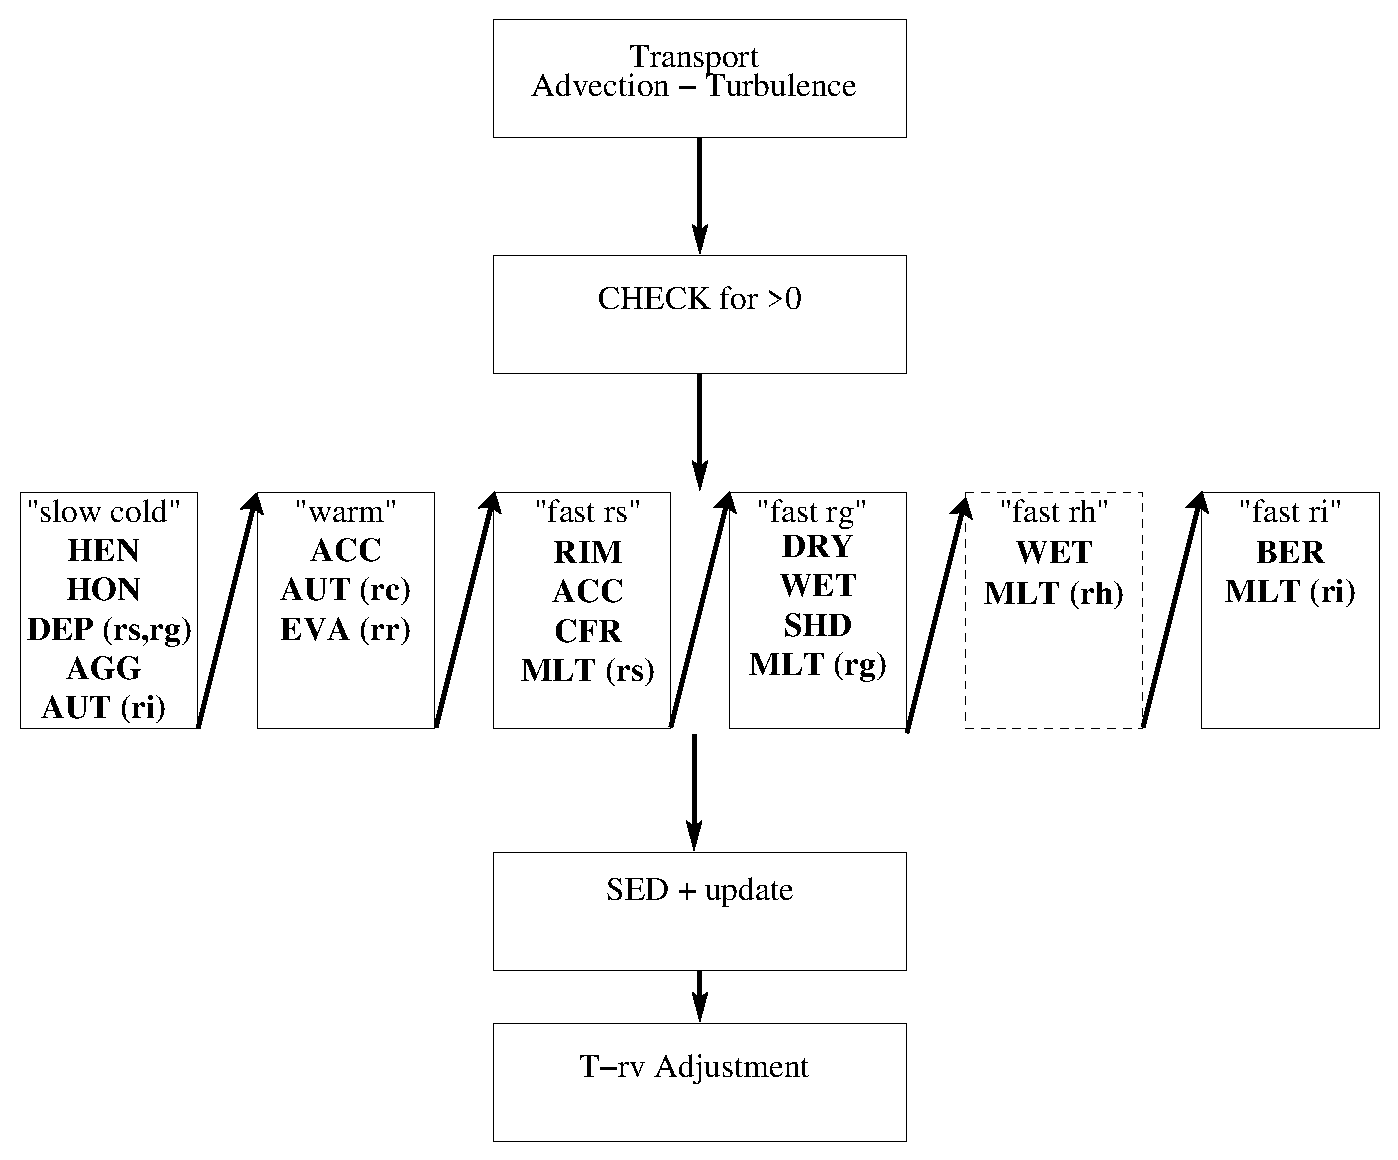
\includegraphics[width=\textwidth]{\EPSDIR/integ_flow.eps}}
\caption{Algorithm of the step-by-step integration of the microphysical processes.}
\label{mixfigalgo}
\end{figure}

%
\subsection{Water vapor adjustments}\label{VAPADJ}
%
All the concurrent microphysical processes involving an exchange of heat and
water vapor on the condensed particles are computed independently each other.
In the warm microphysical scheme an implicit adjustment of the temperature,
water vapor and cloud water fields is performed in order to introduce some
consistency between $\theta$ and $r_v$ with a strict saturation criterium in
clouds leading to a subsequent passive adjustment of $r_c$. A by-product of this
adjustment is the derivation of a condensation/evaporation rate ($RVCNDC$) of
the cloud droplets. In mixed phase clouds the problem is far more complex
because of the presence of cloud droplets and ice (so two species to re-adjust)
and the difficulty of defining unambiguously a single level of saturation. The
solution which has been chosen here is to perform an implicit adjustment as in
Lord et al. (1984) or in Tao et al. (1989) because it seems superior to the
explicit closure exposed in Ferrier (1994) where a simple saturation over ice
is assumed leading to some controversial account of the Bergeron-Findeisen
effect\footnotemark
%
\footnotetext{Note that Krueger et al. (1995) emphasized the fact that the
original adjustment introduced by Lord et al. (1984) cannot reproduce an
implicit Bergeron-Findeisen transfer of mass}
%
and a single correction of $r_i$. In the present scheme
the Bergeron-Findeisen conversion rate ($RCBERI$) is explicitly pre-integrated
and so the traditional linear partition of water vapor correction as a function
of temperature can be subjected to some revision. Another advantage of using an
implicit adjustment scheme in the spirit of that of Lord et al. (1984) is that
it can revert to a classical adjustment
scheme in case of warm cloud ($r_i=0$) or fully glaciated cloud ($r_c=0$).

The major assumptions used in the proposed saturation adjustment scheme are the
following:

\begin{itemize}
\item the saturation vapor mixing ratio ($r_{{vs}_{iw}}$) inside a mixed phase
cloud results from the barycentric formula introduced by Lord et al. (1984)
that is:
%
\be\label{SAT2}
r_{{vs}_{iw}}=\frac{\displaystyle{r_c^* r_{{vs}_{w}}(T)+r_i^* r_{{vs}_{i}}(T)}}
                   {\displaystyle{r_c^* + r_i^* }}
\ee
%
\item the super/sub-saturation adjustment over cloud ice/droplets is made
isobarically and proportionnal to the explicitly estimated cloud water and
cloud ice content, this gives:
%
\be\label{SAT3}
\Delta r_c= r_c-r_c^*=\Delta r_v CND \qquad {\rm and} \qquad
\Delta r_i= r_i-r_i^*=\Delta r_v DEP
\ee
%
\noindent with
%
\be\label{SAT4}
\Delta r_v= r_v^*-r_v=r_v^*-r_{{vs}_{iw}}
\ee
%
\noindent and with
%
\be\label{SAT5}
CND=\frac{\displaystyle{r_c^*}}{\displaystyle{r_c^*+r_i^*}} \qquad
{\rm and} \qquad
DEP=\frac{\displaystyle{r_i^*}}{\displaystyle{r_c^*+r_i^*}}.
\ee
%
So any deficit or excess of water vapor is compensated or absorbed by each
cloudy condensed phase in proportion to their respective content and as a
consequence, $\Delta r_c$ and $\Delta r_i$ have always the same sign. This way
of doing seems raisonnable since once the Bergeron-Findeisen effect is
accounted for, water vapor can be supplied or gathered by $r_c$ and $r_i$ in
proportion to their actual amount\footnotemark
%
\footnotetext{In the remaining text, the starred variables are the most recently
updated (or "guess") variables}
%
.

However, the above adjustment formulation was found to produce to much ice at weakly negative temperature. As a consequence, since the Masdev 4.1 version, the $CND$ and $DEP$ terms are calculated following Tao et al. (1989) as:
\be\label{SAT5NEW}
CND=\frac{T - T_{00} }{T_0 - T_{00} }\qquad
{\rm and} \qquad
DEP=1 - CND \qquad
\ee
with $T_0 = 0^\circ$C  and $T_{00} = 40^\circ$C.

\end{itemize}
The saturation adjustment then proceeds as for Tao et al. (1989) where a
zero-crossing solution of
%
\be\label{SAT6}
\begin{array}{rl}
F(T)&=T-T^*-\frac{\displaystyle{L_v(T) \Delta r_c + L_s(T) \Delta r_i}}
           {\displaystyle{C_{ph}}} \\
  &=T-T^*+\Big({\frac{\displaystyle{L_v(T) CND + L_s(T) DEP}}
                     {\displaystyle{C_{ph}}}}\Big)
                     (r_{{vs}_{iw}}(T)-r_v^*)
\end{array}
\ee
%
\noindent is sought using (\ref{SAT2}) to (\ref{SAT5}) and the non-iterative
algorithm of Langlois (1973) already experienced for the warm microphysical
adjustment is preferred to the first order solution of Tao et al. (1989). Of
course, this adjustment is performed after integrating explicitly all the source
terms in the $\theta$ and the $r_v$ prognostic equations, the cloud condensation
and ice deposition terms excepted.

The procedure used for solving (\ref{SAT6}) is based upon the quasi-second
order expansion of $F(T)=0$, namely\footnotemark
%
\footnotetext{The slow variations of $L_v(T)$ and of $L_s(T)$ with the
temperature are neglected but not those of $r_{{vs}_w}(T)$ and of
$r_{{vs}_i}(T)$.}
%
%
\begin{equation}\label{SAT7}
T \simeq T^*- \dfrac{F(T^*)}{F'(T^*)}
  \Big[ 1+ \dfrac{1}{2} \dfrac{F(T^*)}{F'(T^*)}  \dfrac{F''(T^*)}{F'(T^*)} \Big]
\end{equation}
%

\noindent where
%
\be\label{SAT8}
\begin{array}{rrl}
\Delta_1 &=
\dfrac{F(T^*)}{F'(T^*)}
&= \dfrac { \big [L_v(T^*) CND + L_s(T^*) DEP \big ]
   (r_c^* r_{{vs}_w}(T^*) +r_i^* r_{{vs}_i}(T^*) - (r_c^*+r_i^*) r_v^*) }
     {C_{ph}(r_c^*+r_i^*) + \big [L_v(T^*) CND +L_s(T^*) DEP\big ] \big [r_c^* r'_{{vs}_w}(T^*) + r_i^* r'_{{vs}_i}(T^*)\big ]}, \\
\Delta_2 &=
\dfrac{F''(T^*)}{F'(T^*)}
&= \dfrac { \big [L_v(T^*) CND + L_s(T^*) DEP \big ]
   (r_c^* r''_{{vs}_w}(T^*) +r_i^* r''_{{vs}_i}(T^*)) }
     {C_{ph}(r_c^*+r_i^*) + \big [L_v(T^*) CND +L_s(T^*) DEP\big ] \big [r_c^* r'_{{vs}_w}(T^*) + r_i^* r'_{{vs}_i}(T^*)\big ]}, \\
\end{array}
\ee
%
\noindent and where
%
\be\label{SAT9}
\begin{array}{rl}
r'_{{vs}_w}(T^*) &= A_w(T^*) r_{{vs}_w}(T^*) \Big[1 + \dfrac{r_{{vs}_w}(T^*)}{\epsilon} \Big], \\
r'_{{vs}_i}(T^*) &= A_i(T^*) r_{{vs}_i}(T^*) \Big[1 + \dfrac{r_{{vs}_i}(T^*)}{\epsilon} \Big], \\
r''_{{vs}_w}(T^*) &= r'_{{vs}_w}(T^*) \Big[ \dfrac{A'_w(T^*)}{A_w(T^*)}+A_w(T^*) \big(1+2\dfrac{r_{{vs}_w}(T^*)}{\epsilon}\big) \Big], \\
r''_{{vs}_i}(T^*) &= r'_{{vs}_i}(T^*) \Big[ \dfrac{A'_i(T^*)}{A_i(T^*)}+A_i(T^*) \big(1+2\dfrac{r_{{vs}_i}(T^*)}{\epsilon}\big) \Big]
\end{array}
\ee
%
\noindent with $\epsilon=M_v/M_d$ and
%
\be\label{SAT10}
\begin{array}{rcl}
A_w(T)=\dfrac{\beta_w}{T^2} - \dfrac{\gamma_w}{T}
&\qquad {\rm and} \qquad&
A'_w(T)=-\dfrac{2\beta_w}{T^3} + \dfrac{\gamma_w}{T^2} \\
A_i(T)=\dfrac{\beta_i}{T^2} - \dfrac{\gamma_i}{T}
&\qquad {\rm and} \qquad&
A'_i(T)=-\dfrac{2\beta_i}{T^3} + \dfrac{\gamma_i}{T^2}.
\end{array}
\ee
%

Finally the rates $RVDEPI$ and $RVCNDC$ in the $r_c$ and $r_i$ equations, are
estimated by:
%
\be\label{STA11}
\begin{array}{rrl}
RVDEPI &= \dfrac{(r_v^* - r_{{vs}_{iw}} )DEP}{2\Delta t}
&= \dfrac{C_{ph}}{L_v(T^*) CND + L_s(T^*) DEP} \Big[ -\Delta_1(1+\dfrac{1}{2} \Delta_1 \Delta_2) \Big]
\dfrac{DEP}{2\Delta t}\\
RVCNDC &= \dfrac{(r_v^* - r_{{vs}_{iw}} )CND}{2\Delta t}
&= \dfrac{C_{ph}}{L_v(T^*) CND + L_s(T^*) DEP} \Big[ -\Delta_1(1+\dfrac{1}{2} \Delta_1 \Delta_2) \Big]
\dfrac{CND}{2\Delta t}.
\end{array}
\ee
%


%\vfill
%
\section{References}
\label{section5}
%
\decrefname
B\"ohm, H. P., 1989:
      A general equation for the terminal fall speed of solid hydrometeors.
      {\it J. Atmos. Sci.},
      {\bf 46},
      2419-2427.
\decrefname
Caniaux, G., 1993:
      Param\'etrisation de la glace dans un mod\`ele non-hydrostatique de nuage:
      Application \`a une ligne de grain tropicale.
      {Th\`ese de Doctorat de l'Universit\'e Paul-Sabatier},
      257 pp.
\decrefname
Chaboureau, J.-P., J.-P. Cammas, P. J. Mascart, J.-P. Pinty, and J.-P. Lafore, 2002:
      Mesoscale model cloud scheme assessment using satellite observations.
      {\it J. Geophys. Res.}, {\bf 107(D16)}, 4301, doi:10.1029/2001JD000714.
\decrefname
Chaboureau, J.-P. and J.-P. Pinty, 2006:
      Evaluation of a cirrus parameterization with Meteosat Second Generation.
      {\it Geophys. Res. Let.}, {\bf 33}, L03815, doi:10.1029/2005GL024725.
\decrefname
Cheng, L., and M. English, 1983:
      A relationship between hailstone concentration and size.
      {\it J. Atmos. Sci.},
      {\bf 40},
      204-213.
\decrefname
Chin, H.-N. S., 1994:
      The impact of the ice phase and radiation on a midlatitude squall line
      system.
      {\it J. Atmos. Sci.},
      {\bf 51},
      3320-3343.
\decrefname
Cotton, W. R., G. J. Tripoli, R. M. Rauber and E. A. Mulvihill, 1986:
      Numerical simulations of the effects of varying ice crystal nucleation
      rates and aggregation processes on orographic snowfall.
      {\it J. Climate Appl. Meteor.},
      {\bf 25},
      1658-1680.
\decrefname
Farley, R. D., P. A. Price, H. D. Orville and J. H. Hirsch, 1989:
      On the numerical simulation of graupel/hail initiation via the riming of
      snow in bulk water microphysical cloud models.
      {\it J. Appl. Meteor.},
      {\bf 28},
      1128-1131.
\decrefname
Ferrier, B. S., 1994:
      A double-moment multiple phase four-class bulk ice scheme. Part I:
      description.
      {\it J. Atmos. Sci.},
      {\bf 51},
      249-280.
\decrefname
Ferrier, B. S., W.-K. Tao and J. Simpson, 1995:
      A double-moment multiple phase four-class bulk ice scheme. Part II:
      simulations of convective storms in different large-scale environments and
      comparison with other bulk parameterizations.
      {\it J. Atmos. Sci.},
      {\bf 52},
      1001-1033.
\decrefname
Foote, G. B., and P. S. Du Toit, 1969:
      Terminal velocity of raindrops aloft.
      {\it J. Appl. Meteor.},
      {\bf 8},
      249-253.
\decrefname
Hall, W. D., and H. R. Pruppacher, 1977:
      The survival of ice particles falling from cirrus clouds in subsaturated
      air.
      {\it J. Atmos. Sci.},
      {\bf 33},
      1995-2006.
\decrefname
Hallett, J., and S. C. Mossop, 1974:
      Production of secondary ice particles during the riming process.
      {\it Nature},
      {\bf 249},
      26-28.
\decrefname
Heymsfield, A. J., 1972:
      Ice crystals terminal velocities.
      {\it J. Atmos. Sci.},
      {\bf 29},
      1348-1356.
\decrefname
Heymsfield, A. J. and J. C. Pflaum, 1985:
      A quantitative assessment of the accuracy of techniques for calculating
      graupel growth.
      {\it J. Atmos. Sci.},
      {\bf 42},
      2264-2274.
\decrefname
Houze, R. A. Jr., P. V. Hobbs, P. H. Herzegh and D. B. Parsons, 1979:
      Size distributions of precipitation particles in frontal clouds.
      {\it J. Atmos. Sci.},
      {\bf 36},
      156-162.
\decrefname
Kajikawa, M., and A. J. Heymsfield, 1989:
      Aggregation of ice crystals in cirrus.
      description
      {\it J. Atmos. Sci.},
      {\bf 46},
      3108-3121.
\decrefname
Langlois, W. E., 1973:
      A rapidly convergent procedure for computing large-scale condensation in
      a dynamical weather model.
      {\it Tellus},
      {\bf 25},
      86-87.
\decrefname
Krueger, S. K., Q. Fu, K. N. Liou, and H.-N. S. Chin, 1995:
      Improvements of an ice-phase microphysics parameterization for use in
      numerical simulations of tropical convection.
      {\it J. Appl. Meteor.},
      {\bf 34},
      281-287.
\decrefname
Lascaux, F., E. Richard, and J.-P. Pinty, 2006:
      Numerical simulations of three MAP IOPs and the associated microphysical processes.
     {\it Quart. J. Roy. Meteor. Soc.}, {\bf 132}, 1907-1926.
\decrefname
Lin, Y.-L., R. D. Farley, and H. D. Orville, 1983:
      Bulk parameterization of snow field in a cloud model.
      {\it J. Climate Appl. Meteor.},
      {\bf 22},
      1065-1092.
\decrefname
Locatelli, J. D., and P. V. Hobbs, 1974:
      Fall speeds and masses of solid precipitation particles.
      {\it J. Geophys. Res.},
      {\bf 79D},
      2185-2197.
\decrefname
Lord, S. J., H. E. Willoughby, and J. M. Piotrowicz, 1984:
      Role of a parameterized ice-phase microphysics in an axisymmetric
      non-hydrostatic tropical  cyclone model.
      {\it J. Atmos. Sci.},
      {\bf 41},
      2836-2848.
\decrefname
Nelson, S. P., 1983:
      The influence of storm flow structureon hail growth.
      {\it J. Atmos. Sci.},
      {\bf 40},
      1965-1983.
\decrefname
Mc Cumber, M., W.-K. Tao, J. Simpson, R. Penc, and S. T. Soong, 1991:
      Comparaison of ice-phase microphysical parameterization schemes using
      numerical simulations of tropical convection.
      {\it J. Appl. Meteor.},
      {\bf 30},
      985-1004.
\decrefname
Mc Farquhar, G. M., A. J. Heymsfield, 1997:
      Parameterization of tropical cirrus ice crystal size distributions and
      implications for radiative transfer: Results from CEPEX
      {\it J. Atmos. Sci.},
      {\bf 54},
      2187-2200.
\decrefname
Masson, B. J., 1956:
      On the melting of hailstones.
      {\it Quart. J. R. Met. Soc.},
      {\bf 82},
      209-216.
\decrefname
Meyers, M. P., P. J. DeMott, and W. R. Cotton, 1992:
      New primary ice-nucleation parameterizations in an explicit cloud model.
      {\it J. Appl. Meteor.},
      {\bf 31},
      708-721.
\decrefname
Meyers, M. P., R. L. Walko, J. Y. Harrington and W. R. Cotton, 1996:
      New RAMS cloud microphysics parameterization. Part II: The two-moment
      scheme.
      {\it submitted to Atm. Res.}
\decrefname
Murakami, M., 1990:
      Numerical modeling of dynamical and microphysical evolution of an isolated
      convective cloud -the 19 July 1981 CCOPE cloud.
      {\it J. Meteor. Soc. Japan},
      {\bf 68},
      107-128.
\decrefname
Musil, D. J., 1970:
      Computer modeling of hailstone growth in feeder clouds.
      {\it J. Atmos. Sci.},
      {\bf 27},
      474-482.
\decrefname
Passarelli, R. E., Jr., 1978:
      An approximate analytical model of the vapor deposition and aggregation
      growth of snow.
      {\it J. Atmos. Sci.},
      {\bf 35},
      118-124.
\decrefname
Pruppacher, H. R., and J. D. Klett, 1978:
      {\it Microphysics of Clouds and Precipitation}.
      Reidel,714 pp.
\decrefname
Rutledge, S. A. and P. V. Hobbs, 1983:
      The mesoscale and microscale structure and organization of clouds and
      precipitation in midlatitude cyclones. Part VIII: A model for the
      "Seeder-Feeder" process in warm-frontal rainbands.
      {\it J. Atmos. Sci.},
      {\bf 40},
      1185-1206.
\decrefname
Rutledge, S. A. and P. V. Hobbs, 1984:
      The mesoscale and microscale structure and organization of clouds and
      precipitation in midlatitude cyclones. Part XII: A diagnostic modeling
      study of precipitation development in narrow cold-frontal rainbands.
      {\it J. Atmos. Sci.},
      {\bf 41},
      2949-2972.
\decrefname
Ryan, B. F., 2000: A bulk parameterization of the ice particle size
      distribution and the optical properties in ice clouds,
      {\it J. Atmos. Sci.}, {\bf 57}, 1436-1451.
\decrefname
Starr, D. O'C. and S. K. Cox, 1985:
      Cirrus clouds. Part I: A cirrus cloud model.
      {\it J. Atmos. Sci.},
      {\bf 42},
      2663-2681.
\decrefname
Sue Chen, and W. R. Cotton, 1988:
      The sensitivity of a simulated extratropical mesoscale convective system
      to longwave radiation and ice-phase microphysics.
      {\it J. Atmos. Sci.},
      {\bf 45},
      3897-3910.
\decrefname
Tao, W.-K., J. Simpson, and M. Mc Cumber, 1989:
      An ice-water saturation adjustment.
      {\it Mon. Wea. Rev.},
      {\bf 117},
      231-235.
\decrefname
Tripoli, G. J., P. J. Flatau, and W. R. Cotton, 1988:
      Generalized microphysics scheme for use in mesoscale cloud model.
      {\it Preprints 10$^{th}$ International Cloud Physics Conference}.
      Bad-Homburg. FRG August, 1988,
      109-111.
\decrefname
Walko, R. L., W. R. Cotton, M. P. Meyers, and J. Y. Harrington, 1995:
      New RAMS cloud microphysics parameterization. Part I: The single-moment
      scheme.
      {\it Atm. Res.},
      {\bf 38},
      29-62.
\decrefname
Yang M.-J. and R. A. Houze, 1995:
      Sensitivity of squall-line rear inflow to ice microphysics and
      environmental humidity.
      {\it Mon. Wea. Rev.},
      {\bf 123},
      3175-3193.
\decrefname
Ziegler, C. L., 1985:
      Retrieval of thermal and microphysical variables in observed convective
      storms. Part I: Model development and preliminary testing.
      {\it J. Atmos. Sci.},
      {\bf 42},
      1487-1509.
\decrefname
Ziegler, C. L., 1988:
      Retrieval of thermal and microphysical variables in observed convective
      storms. Part II: Sensitivity of cloud processes to variation of the
      microphysical parameterization.
      {\it J. Atmos. Sci.},
      {\bf 45},
      1072-1090.
\decrefname

%\end{document}

%%%%%%%%%%%%%%%%%%%%%%%%%%%%%%%%%%%%%%%%%%%%%%%%%%%%%%%%%%%%%%%%%%%%%%%%%%%%%%%
%%%%%%%%%%%%%%%%%%%%%%%%%%%%%%%%%%%%%%%%%%%%%%%%%%%%%%%%%%%%%%%%%%%%%%%%%%%%%%
%%%%%%%%%%%%%%%%%%%%%%%%%%%%%%%%%%%%%%%%%%%%%%%%%%%%%%%%%%%%%%%%%%%%%%%%%%%%%%
%%%%%%%%%%%%%%%%%%%%%%%%  END OF ICE MICROPHYSICS %%%%%%%%%%%%%%%%%%%%%%%%%%%
%%%%%%%%%%%%%%%%%%%%%%%%%%%%%%%%%%%%%%%%%%%%%%%%%%%%%%%%%%%%%%%%%%%%%%%%%%%%%%
%%%%%%%%%%%%%%%%%%%%%%%%%%%%%%%%%%%%%%%%%%%%%%%%%%%%%%%%%%%%%%%%%%%%%%%%%%%%%%


